%%
%% 'BScWIMEngl.tex'
%%
%% LaTeX template for Bachelor theses at the faculty WIM
%% of Mannheim University
%%
%% copyleft (2012-2014) by J. Berger, T. Christen, and J. Potthoff	
%%

%%fleqn leftalignes equations
\documentclass[11pt, a4paper]{book}
\usepackage{./macros/dinaA4}
\usepackage{./macros/BScMacros}
\usepackage{./macros/BScTitle}

\usepackage{tikz,tikz-cd}
\usetikzlibrary{
    shapes,% for the rectangle
    chains,% provides the chains
    scopes,
    arrows,%
    matrix,%
    positioning,% wg. " of "
    scopes,%
    decorations.pathmorphing,% /pgf/decoration/random steps | erste Graphik
    shadows%
}% allows to replace \begin{scope} \end{scope} with {}

\newcommand{\vsubseteq}{\rotatebox[origin=c]{-90}{\(\subseteq\)}}

\usepackage[style=authoryear, backend=biber]{biblatex}
\addbibresource{./chapter/literature.bib}

\usepackage[draft]{fixme} %final removes annotations 
\fxsetup{theme=color}
%%\fxnote{some note} ,\fxwarning{}, \fxerror{}, \fxfatal{} <- does not allow [final] to compile

%%
%% je nach Betriebssystem und Editor muss die
%% Behandlung von Sonderzeichen wie Umlauten
%% eingestellt werden - dazu unten das richtige 
%% (TeX-Guru fragen!) Paket auswaehlen 
%% (d.h., das "%" Zeichen am Anfang der Zeile entfernen)
%% (man geht auf "Nummer Sicher", indem man
%% Umlaute wie \"a eingibt, {\ss} fuer Eszett -
%% dann braucht man keins der Pakete unten)
%%
%\usepackage[cp850]{inputenc} 
%\usepackage[latin1]{inputenc} 
%\usepackage[ansinew]{inputenc}
\usepackage[utf8]{inputenc}
%\usepackage{ucs}
%\usepackage[utf8x]{inputenc}

\usepackage{csquotes}

%%
%% Font auswaehlen: '\TimesFont' auskommentiert -> computer modern
%% '\TimesFont' aktiv -> Textfont: times, Mathfont: computer modern
%%
%\TimesFont
%%
%% ein- oder doppelseitiger Satz
%%
%\onesided
\twosided
%%
%% persoenliche Angaben
%%
\firstLastName{Felix Benning}
\birthdate{27.11.1996}
\birthplace{Nürtingen}
\MatNr{1501817}
\titellineI{Reinforcement Learning}
%\titellineII{}
%\titellineIII{}
%\subtitellineI{}
%\subtitellineII{}
\Supervisor{Prof. Dr. Leif Döring}
\DueDate{11.05.2019}


\begin{document}
\listoffixmes
\frontmatter
\titelpage
%%
%% eidestattliche Erklaerung
%%
\chapter*{Declaration of Authorship}
\thispagestyle{empty}

I hereby declare that the thesis submitted is my own unaided work. All direct or indirect sources used are acknowledged as references.

\vspace{.5\baselineskip}
This thesis was not previously presented to another examination board and has not been published.

\vspace{4\baselineskip}
\begin{center}
\parbox{.8\textwidth}{City, Date \hfill Signature}
\end{center}

\endinput

\cleardoublepage
%%
%% Vorwort
%%
%\chapter{Preface}

\endinput

\setcounter{tocdepth}{1}
%%
%% Inhaltsverzeichnis
%%
\tableofcontents
%%
%% Einleitung
%% (nicht alle Autoren trennen Vorwort und Einleitung,
%%  manche setzen die Einleitung als erstes Kapitel
%%  nach "\mainmatter")
%%
%% !TEX root = ../BScWIMEngl.tex

\chapter{Introduction}
    Let us consider a system to be a intelligent, if it collects information from its sensors and transforms this information into an ``appropriate'' response. Then the question where this input comes from (eyes, ears, cameras, etc.), or what kind of input it is (visual, audio, etc.), is as irrelevant for this definition, as the question what a response is (motor activity, sound, etc.). An intelligent system is simply a function mapping inputs to ``appropriate'' outputs.  The question what ``appropriate'' means, is in contrast a lot more important and difficult to answer. But if we assume that there exists a ``correct'' response, then this correct response is itself a function from the input space to the output space. Artificial intelligence is therefore simply an artificial implementation of this correct response function. 

    If we have complete knowledge of this function, we can encode this function as an executable program manually. But more often than not, we do not really understand the rules according to which the inputs are supposed to be transformed into outputs. 

    For this reason we might want a machine to ``learn'' these rules by itself, i.e. we want it to approximate the correct response function. There are two larger subcategories in this category of \emph{machine learning}. 
    
    In \emph{supervised learning} we do not know the correct response function, but we know the correct response for certain inputs intuitively. An example for this case is image classification of animals. There, we do not know how the input (pixels of the picture) map to the output (name of the animal), but we can tell for a given picture what animal is depicted intuitively, i.e. we can provide examples of the correct response function to the learning algorithm. Supervised Learning is therefore concerned with generalization from examples. And while approximating a function with a finite sample of (error prone) function evaluations is a relatively old problem in numerical analysis and statistics, supervised learning is often associated with more recent approaches like artificial neuronal networks. 

    While we are still able to provide examples in supervised learning, \emph{unsupervised learning} has to work with even less. This category includes clustering and principle component analysis, as well as \emph{reinforcement learning}. Reinforcement learning is applied to problems, where we ``know the correct response if we see it'', but can not provide examples ourselves. This is for example the case with walking. We know how walking looks like, but we have a hard time giving an example for the correct output signals sent to the motors in the leg. It is also used in cases where we do not know the correct response and have never seen it, but are able to compare different response functions. Examples range from games like chess, to profit maximization of a company. 

    In general reinforcement learning is used in cases, where humans or the environment in general can rate the solution, and provide rewards for good outcomes. Similar to the conditioning of animals, desirable actions are \emph{reinforced} with rewards. 

    But in order to write algorithms, which maximize their rewards, we first need to formulate the relationship of possibly delayed rewards with actions (outputs) of the learning algorithm in certain states (given certain inputs). The model for this relationship -- which virtually all modern reinforcement learning algorithms are based on -- is the Markov Decision Process. 
    
    We will therefore introduce this model and its properties in the first chapter, continue with a review of common reinforcement algorithms in the second chapter, and explore the relation between the theory of stochastic approximation and reinforcement learning in the third chapter, which yields proofs of convergence to the optimal policy for a number of reinforcement algorithms. \fxnote{check}
\endinput

\mainmatter
%%
%% eigentliche Kapitel der Arbeit
%%
%\documentclass[11pt, a4paper]{book}

\usepackage{tikz,tikz-cd}
\usetikzlibrary{
    shapes,% for the rectangle
    chains,% provides the chains
    scopes,
    arrows,%
    matrix,%
    positioning,% wg. " of "
    scopes,%
    decorations.pathmorphing,% /pgf/decoration/random steps | erste Graphik
    shadows%
}% allows to replace \begin{scope} \end{scope} with {}


\begin{document}
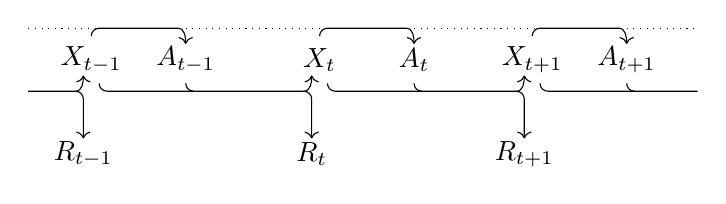
\begin{tikzpicture}
    \draw[dotted] (-3.7,0.4) -- (-2.8,0.4);

    \draw[->] (-3.7, -0.4) %%% transition stub beginning
    to [out=0,in=180] (-3.1, -0.4)
    to [out=0,in=270] (-3, -0.2);

    \draw[->] (-3.1, -0.4) %%% to R_{t-1}
    to [out=0,in=90] (-3,-0.5)
    to [out=270, in=90] (-3,-1);

    \draw (-3,-1.2) node {\(R_{t-1}\)};
    \draw (-2.9,0) node {\(X_{t-1}\)};

    \draw[->] (-2.9,0.3) %%% X_{t-1} to A_{t-1}
    to [out=90,in=180] (-2.8, 0.4) 
    to [out=0,in=180] (-1.8,0.4)
    to [out=0,in=90] (-1.7,0.2);

    \draw[dotted] (-1.7,0.4) -- (0.1,0.4);

    \draw (-1.7,0) node {\(A_{t-1}\)};

    \draw (-1.7, -0.3) %%% join transition 
    to [out=270,in=180] (-1.6,-0.4);

    \draw[->] (-2.8, -0.3) %%% X_{t-1} to X_t transition
    to [out=270,in=180] (-2.7, -0.4) 
    to [out=0,in=180] (-0.2, -0.4)
    to [out=0,in=270] (-0.1, -0.2);

    \draw[->] (-0.2, -0.4) %%% to R_t
    to [out=0,in=90] (-0.1,-0.5)
    to [out=270, in=90] (-0.1,-1);

    \draw (-0.1,-1.2) node {\(R_t\)};
    \draw (0,0) node {\(X_t\)};
    
    \draw[->] (0,0.3)  %%% X_t to A_t
    to [out=90,in=180] (0.1, 0.4) 
    to [out=0,in=180] (1.1,0.4)
    to [out=0,in=90] (1.2,0.2); 

    \draw[dotted] (1.2,0.4) -- (2.8,0.4);
 
    \draw (1.2,0) node {\(A_t\)};

    \draw (1.2, -0.3) %%% join transition
    to [out=270,in=180] (1.3,-0.4);

    \draw[->] (0.1, -0.3) %%% X_t to X_{t+1} transition
    to [out=270,in=180] (0.2, -0.4) 
    to [out=0,in=180] (2.5, -0.4)
    to [out=0,in=270] (2.6, -0.2);

    \draw[->] (2.5, -0.4) %%% to R_{t+1}
    to [out=0,in=90] (2.6,-0.5)
    to [out=270, in=90] (2.6,-1);

    \draw (2.6,-1.2) node {\(R_{t+1}\)};
    \draw (2.7,0) node {\(X_{t+1}\)};

    \draw[->] (2.7,0.3)  %%% X_{t+1} to A_{t+1}
    to [out=90,in=180] (2.8, 0.4) 
    to [out=0,in=180] (3.8,0.4)
    to [out=0,in=90] (3.9,0.2); 

    \draw[dotted] (3.9,0.4) -- (4.8,0.4);

    \draw (3.9,0) node {\(A_{t+1}\)};

    \draw (3.9, -0.3) %%% join transition stub
    to [out=270,in=180] (4,-0.4);

    \draw (2.8, -0.3) %%% X_{t+1} transition stub end
    to [out=270,in=180] (2.9, -0.4) 
    to [out=0,in=180] (4.8, -0.4);
\end{tikzpicture}
\end{document}


\chapter{Markov Decision Processes}
\begin{definition}(Kernel)
	\((Y,\cA_Y), (X,\cA_X)\) measure spaces\\
	 \(\lambda\colon X\times\cA_Y\to \R\) is a \emph{(probability) kernel} \(
	 :\iff \begin{aligned}[t]
	 &\lambda(\cdot,A)\colon x\mapsto \lambda(x,A) \text{ measurable}\\
	 &\lambda(x,\cdot)\colon A\mapsto \lambda(x,A) \text{ a (prob.) measure}
	 \end{aligned}
	  \)\\
	  Since we will interpret probability kernels as distributions over \(Y\) given a  certain condition \(X\), the notation \(\lambda(\cdot\mid x) \coloneqq \lambda(x,\cdot)\) helps this intuition. 
\end{definition}
\begin{definition}(Markov Decision Process - MDP)\\
\(\cM=(\cX,\cA,\cP_0) \), with:
	
\begin{tabular}{l l l}
	\(\cX\) & countable (finite) set of states&\\
	\(\cA\) & countable (finite) set of actions &\\
	\multicolumn{2}{l}{
		\(
		\begin{cases}
		\cX\times \cA \to \pmeas(\cX\times\R)\\
		(x,a)\mapsto \cP_0(\cdot \mid x,a)
		\end{cases}
		\)
	}  &
	\parbox[h]{17em}{
		\emph{transition probability kernel} \\
		\(\pmeas(\cX\times\R) \) the set of probability measures on \(\cX\times\R \), \\
		\(\cX\) represents the next states,\\
		\(\R\) the payoffs
	}
	\end{tabular}\\
is a \emph{(finite) Markov Decision Process}.\\
Together with a discount factor \(\gamma\in[0,1]\) it is a:\\
\begin{tabular}{l l}
	\emph{discounted reward} MDP & \(\gamma <1 \)\\
	\emph{undiscounted reward} MDP & \(\gamma=1 \)
\end{tabular}\\
For \((Y_{(x,a)}, R_{(x,a)})\sim \cP_0(\cdot\mid x,a) \) a random variable, is
\[r(x,a)\coloneqq \E[R_{(x,a)}] \quad\text{ the \emph{immediate reward function}}\]
An MDP is \emph{evaluated} as follows:\\
1. Select the initial state \(X_0\) an \(\cX\)-valued random variable.\\ 
2. \((A_t, t\in \N)\) action selection rules (behaviors) will be discussed later, for now simply assume \(\cA\)-valued random variables.\\
3. Select inductively: \((X_{t+1}, R_{t+1})\sim\cP_0(\cdot\mid X_t, A_t)\) with the markov property, i.e.:
\begin{align*} 
&\Pr[(X_{t+1},R_{t+1})=(x,r) \mid (X_t,A_t)=(x_t,a_t),\dots, (X_0,A_0)=(x_0,a_0)]\\
&=\Pr[(X_{t+1}, R_{t+1})=(x,r)\mid (X_t,A_t)=(x_t,a_t)]
\end{align*}
resulting in the stochastic process \(((X_t,A_t,R_{t+1}), t\geq 0)\), which allows to define the \emph{return}:
\[\cR\coloneqq\sum_{t=0}^{\infty}\gamma^t R_{t+1}\]
\end{definition}
%(

\begin{remark}
\((X_{t+1}, R_{t+1})\sim\cP_0(\cdot\mid X_t, A_t)\) with the markov property is well defined, i.e.:
\begin{align*}
	&\exists (X_{t+1}, R_{t+1})\ \cX\times\R\text{-valued random variable}: \\ 
	&(X_{t+1}, R_{t+1})\sim\cP_0(\cdot\mid X_t, A_t) \text{ and satisfies the markov property}
\end{align*}
\end{remark}
\begin{proof}
	%TODO
\end{proof}
\begin{remark}\leavevmode
\begin{enumerate}
	\item From now on we assume that \(\forall (x,a)\in\cX\times\cA:|R_{(x,a)}|\le R\in\R\) almost surely. This also implies: 			\(
	\begin{aligned}[t]
		&\|r\|_{\infty}=\sup_{(x,a)\in\cX\times\cA}|\E[R_{(x,a)}]|\le R\\
		&|\cR|\le\sum_{t=0}^\infty \gamma^t |R_{t+1}|\le \frac{R}{1-\gamma} \text{ a.s.}
	\end{aligned}
	\)
	\item Sometimes not all actions make sense in all states. A simple fix would be to set the immediate reward functions for those actions very low, or (if possible) redirect them to the closest possible action. \\
	A more formal approach would be to introduce an additional mapping, which assigns the set of admissible actions to each state \(\cX\to\cP(\cA)\), or alternatively define a (binary) relation on \(\cX\times\cA\).
	\item If there is just one admissible action in every state, the MDP is equivalent to a normal Markov Process.
	\item Instead of a transition probability kernel \(\cP_0\), sometimes a \emph{transition function} f with a and an exogenous random element \(D_t\) (e.g. Demand) is used to define the next state and reward: \((X_{t+1},R_{t+1})=f(X_t,A_t,D_t)\) 
\end{enumerate}
\end{remark}
\begin{definition}\(\cM=(\cX,\cA,\cP_0)\) a MDP\\
	\(x\in\cX\) is a \emph{terminal (absorbing)} state \(:\iff \forall s\in\N: \Pr(X_{t+s}=x\mid X_t=x)=1\)\\
	An MDP with such states is called \emph{episodic}.\\
	An \emph{episode} is the random time period \((1,\dots,T)\) until a terminal state is reached.
\end{definition}
\begin{remark}\leavevmode
	\begin{itemize}
		\item The reward in a terminal state is by convention zero, i.e. \(x\) terminal state implies \(\forall a\in\cA: R_{(x,a)}=0\).
		\item Episodic MDPs are often undiscounted
	\end{itemize}	
\end{remark}
\begin{definition}\(\cM=(\cX,\cA,\cP_0)\) a MDP\\
	 An \(A_t\) selection-rule \(\pi=(\pi_t,t\in\N_0)\) is called \emph{behavior}, where
	 \[ 
	 	\pi_t\colon
	 	\begin{cases}
	 		((\cX\times\cA\times\R)^t\times\cX)\times\cP(\cA) \to \R \\
	 		(y,A)\mapsto \pi_t(A\mid y)
	 	\end{cases} \text{ is a probability kernel}
	 \]
	 and \(A_t\sim \pi_t(\cdot\mid (X_0,A_0,R_1), \dots,(X_{t-1},A_{t-1},R_t),X_t))\)\\
	 Special cases:
	 \begin{enumerate}
	 	\item \emph{Determinisitic stationary policies} specified with some abuse of notation:
	 	\[\leavevmode \pi\colon\cX\to\cA \text{ with }A_t=\pi(X_t)\]
	 	\item \emph{(Stochastic) stationary policies} specified by:
	 	\[\pi\colon \begin{cases}
	 	\cX\times\cP(\cA)\to\R\\
	 	(x,A)\mapsto \pi(A\mid x)
	 	\end{cases} \text{ with } A_t\sim\pi(\cdot\mid x)
	 	\]
	 \end{enumerate}
	 \(\statPolicy\) is the \emph{set of (stoch.) stationary policies}, \\ 
	 \(\detPolicy\) is the \emph{set of deterministic stationary policies} (note \(\detPolicy\subseteq\statPolicy \))
\end{definition}
\begin{remark}
A stationary policy induces a \emph{time-homogenous} markov chain.
\end{remark}
\begin{definition}(Markov Reward Process - MRP)
%TODO
\end{definition}
\section{Value functions}
The goal in this section is to
\begin{itemize}[itemsep=0pt, topsep=1pt]
\item define Value functions which assign states (and actions) a value, which allow the agent to make a more nuanced decisions than comparing immediate rewards of different actions
\item explore the relation of different value functions
\item show uniqueness of optimal value functions with the Banach fixpoint theorem, yielding a simple approximation methode along the way
\item demonstrate that in MDPs deterministic stationary policies are generally a large enough set of policies to choose from
 \end{itemize}
\begin{definition}\(\cM=(\cX,\cA,\cP_0)\) MDP, \(\pi\) Behavior\\
Select \(X_0\) such that \(\forall x\in\cX:\Pr(X_0=x)>0\) and evaluate the MDP with
\(((X_t,A_t,R_{t+1}), t\in \N_0)\) the resulting stoch. process.\\
\def\arraystretch{3}
\[
\begin{array}{l l}
	V^\pi\colon
	\begin{cases}
		\cX\to\R\\
		x\mapsto \E[\cR\mid X_0=x]
	\end{cases} 
	& \text{is the \emph{value function} for } \pi \footnotemark\\
	Q^\pi\colon
	\begin{cases}
		\cX\times\cA\to\R\\
		(x,a)\mapsto \E[\cR\mid X_0=x, A_0=a]
	\end{cases}
	& \text{is the \emph{action value function} for } \pi \footnotemark\\
	V^*\colon
	\begin{cases}
		\cX\to\R\\
		x\mapsto \sup\limits_{\pi\text{ Behav.}} V^\pi(x)
	\end{cases} 
	& \text{is the \emph{optimal value function}}\\
	Q^*\colon
	\begin{cases}
		\cX\times\cA\to\R\\
		(x,a)\mapsto \sup\limits_{\pi\text{ Behav.}} Q^\pi(x,a)
	\end{cases}
	& \text{is the \emph{optimal action value function}}
\end{array}
\]
\(\pi\) is \emph{optimal} \(:\iff V^*=V^\pi\)
\end{definition}
\footnotetext[1]{Well defined because \(\Pr(X_0=x)>0\)}
\footnotetext{Well defined because \(A_1\sim \pi_1(\cdot\mid (x,a,r_0), x_1)\) is defined for all \(a\) regardless of \(\pi_0\)}

\begin{remark}
With the distribution of \(X_0\) set (or \(X_0\) being realized with a fixed value \(x\)), the distribution of \(X_t, A_t,R_{t+1}\) is determined for all \(t\in\N_0\). The conditional expectation is thus unique for a given \(X_0=x\), for all possible realizations of the MDP with a given behavior. \\
This means \(V^\pi, Q^\pi\) are well defined.
\end{remark}


\begin{definition}\(\cM=(\cX,\cA,\cP_0)\) MDP\\
Sometimes we don't care about the probability distribution of the reward, so we define:
	\[
	p\colon 
	\begin{cases}
		\cX\times\cA\times\cP(\cX)\to\R\\
		(x,a,Y)\mapsto \cP_0(Y\times\R\mid x,a)
	\end{cases}\text{ the \emph{\underline{state} transition kernel}.}
	\] 
And use the notation \(p(y\mid x,a)\coloneqq p(\{y\}\mid x,a)\) with \((x,a,y)\in\cX\times\cA\times\cX\)
\end{definition}


\begin{prop}\label{expand Q^pi}\(\cM=(\cX,\cA,\cP_0)\) MDP, \(\pi\in\detPolicy\) 
	\[Q^\pi(x,a)=r(x,a)+\gamma\sum_{y\in\cX}p(y\mid x,a)V^\pi(y)	\]
\end{prop}

\begin{proof}
\begin{align*}
Q^\pi &= \E[\cR(\pi)\mid X_0=x, A_0=a]\\
&=\E[R_1(\pi)\mid X_0=x,A_0=a]+\gamma\E\left[\sum_{t=0}^\infty\gamma^t R_{t+2}(\pi)\middle| X_0=x,A_0=a\right]\\
&=\E[R_{(x,a)}] 
 + \gamma \sum_{y\in\cX}\E\left[\sum_{t=0}^\infty\gamma^t R_{t+2}(\pi) \middle| X_0=x,A_0=a, X_1=y\right]p(y\mid x, a)\\
&\lxeq{\text{Markov}} r(x,a)
 + \gamma\sum_{y\in\cX}\underbracket{\E\left[\sum_{t=0}^\infty\gamma^t R_{t+2}(\pi)\middle| X_1=y, A_1=\pi(y)\right]}_{
 \begin{aligned}
 	&= \E\left[\sum_{t=0}^\infty\gamma^t R_{t+2}(\pi)\middle| X_1=y \right] \\
 	&\lxeq{(*)} \E\left[\sum_{t=0}^\infty\gamma^t \tilde{R}_{t+1}(\pi)\middle| \tilde{X}_0=y \right]=V^\pi(y)
 \end{aligned}
 }
 p(y\mid x, a)
\end{align*}
\((*)\) Rename: \(\tilde{X}_{t}\coloneqq X_{t+1}, \tilde{A}_t\coloneqq A_{t+1},\tilde{R}_{t}\coloneqq R_{t+1}\), then \((\tilde{X}_t,\tilde{A}_t,\tilde{R}_{t+1}, t\in\N_0)\) is an evaluation of the MDP with the (stationary) policy \(\pi\)
\end{proof}


\begin{corollary}\label{V^pi,Q^pi relation}  \(\cM=(\cX,\cA,\cP_0)\) MDP, \(\pi\in\detPolicy\) 
\begin{align*}
	V^\pi(x)&=Q^\pi(x,\pi(x))\\
	 &=r(x,\pi(x))+\gamma\sum\limits_{y\in\cX}p(y\mid x,\pi(x))V^\pi(y) 
\end{align*}
\end{corollary}

\begin{proof}
Since \(\pi\) is a deterministic stationary policy:
\[V^\pi(x)=\E[\cR(\pi)\mid X_0=x]=\E[\cR(\pi)\mid X_0=x, A_0=\pi(x)]=Q^\pi(x,\pi(x))\]
The rest follows from \ref{expand Q^pi}
\end{proof}

\begin{definition}\(\cM=(\cX,\cA,\cP_0)\) MDP, \(\pi\in\detPolicy\) \\
The mapping \(T^\pi\colon\R^\cX\to\R^\cX\) with:
	\[
	T^\pi V(x)\coloneqq r(x,\pi(x))+\gamma\sum_{y\in\cX}p(y\mid x,\pi(x)) V(y)\qquad V\in\R^\cX, x\in\cX
	\]
is called the \emph{Bellman Operator}
\end{definition}


\begin{remark}\leavevmode
	\begin{enumerate}[label=\arabic*.]
	\item \(\forall\pi\in\detPolicy : T^\pi V^\pi=V^\pi\) (c.f. \ref{V^pi,Q^pi relation})
	\item\label{num:2} \(T^\pi\) meets the requirements of the Banach fixed-point theorem for \({\gamma<1}\), this implies that \(V^\pi\) for \(\pi\in\detPolicy\)
	is a \emph{unique} fixpoint and can be approximated with the canonical iteration
	\item \(T^\pi\) is an affine operator
	\item\label{num:4} \(W_1,W_2\in\R^\cX\), write \(W_1 \le W_2\) for \(\forall x\in\cX:W_1(x)\le W_2(x)\), then:
	\[W_1\le W_2 \implies T^\pi W_1\le T^\pi W_2\]
	\end{enumerate}
\end{remark}

\begin{proof}
\ref{num:2} \((\R^\cX, \|\cdot\|_\infty)\) is a non-empty, complete metric space and the mapping maps onto itself. It is left to show, that \(T^\pi\) is a contraction. Be \(V,W\in\R^\cX\):
\begin{align*}
	\|T^\pi V -T^\pi W\|_\infty &=\|\gamma\sum_{y\in\cX} p(y\mid \cdot,\pi(\cdot)) (V(y)-W(y))\|_\infty\\
	&\le\gamma \sup_{x\in\cX}\left\{ \sum_{y\in\cX} p(y\mid x,\pi(x)) \|V-W\|_\infty \right\}\\
	&=\gamma \|V-W\|_\infty  \sup_{x\in\cX}\underbracket{\left\{ \sum_{y\in\cX} p(y\mid x,\pi(x)) \right\}}_{=1}\\
	&=\gamma \|V-W\|_\infty 
\end{align*}
\ref{num:4} Be \(W_1,W_2\in\R^\cX\), \(W_1\le W_2\) and \(x\in\cX\):
\begin{align*}
	T^\pi W_2 (x) - T^\pi W_1(x) 
	= \gamma \sum_{y\in\cX} p(y\mid x,\pi(x)) \underbracket{(W_2(y)-W_1(y))}_{\ge 0} 
	\ge 0
\end{align*}
\end{proof}


\begin{definition}\(\cM=(\cX,\cA,\cP_0)\) MDP
\begin{align*}
	\tilde{V}(x)&\coloneqq \sup_{\pi\in\detPolicy} V^\pi(x)\\
	\tilde{Q}(x,a)&\coloneqq\sup_{\pi\in\detPolicy}Q^\pi(x,a)
\end{align*}
\end{definition}


\begin{definition}\(\cM=(\cX,\cA,\cP_0)\) MDP\\
The mapping \(T^*\colon\R^\cX\to\R^\cX\) with:
	\[
	 T^* V(x)\coloneqq \sup_{a\in\cA}\left\{r(x,a)+\sum_{y\in\cX}p(y\mid x,a) V(y)\right\} \qquad V\in\R^\cX, x\in\cX
	\]
is called the \emph{Bellman Optimality Operator}
\end{definition}


\begin{lemma}\label{V*,Q* relation}\(\cM=(\cX,\cA,\cP_0)\) MDP
\begin{enumerate}[label=\textbf{(\roman*)},font=\normalfont]
\item\label{i:1} \(\tilde{V}(x)=\sup\limits_{a\in\cA} \tilde{Q}(x,a)\)
\item\label{i:2} \( \tilde{Q}(x,a) = r(x,a)+\gamma\sum\limits_{y\in\cX}p(y\mid x,a)\tilde{V}(y) \)
\item\label{i:3} \(V^*(x)=\sup\limits_{a\in\cA}Q^*(x,a)\)
\item\label{i:4} \(Q^*(x,a)=r(x,a)+\gamma \sum\limits_{y\in\cX}p(y\mid x,a) V^*(y)\)
\end{enumerate}
\end{lemma}

\begin{proof} \ref{i:1}, \ref{i:2}
By \ref{V^pi,Q^pi relation} we know \(V^\pi(x)=Q^\pi(x,\pi(x))\) thus:
\begin{align*}
	\tilde{V}(x) =\sup_{\pi \in \detPolicy} V^\pi(x) \le \sup_{a\in \cA}\sup_{\pi\in\detPolicy} Q^\pi(x,a)
	=\sup_{a\in \cA} \tilde{Q}(x,a)
\end{align*}
Because of \ref{expand Q^pi} we know:
\begin{align*}
	\tilde{Q}(x,a)&=\sup_{\pi\in\detPolicy}Q^\pi(x,a) \\
	&= \sup_{\pi\in\detPolicy} \left\{ r(x,a)+\gamma\sum\limits_{y\in\cX}p(y\mid x,a) V^\pi(y) \right\}\\
	&\le r(x,a)+\gamma\sum\limits_{y\in\cX}p(y\mid x,a) \underbracket{\sup_{\pi\in\detPolicy} V^\pi(y)}_{\tilde{V}(y)} \\
\end{align*}
%TODO
\end{proof}


\begin{corollary}
	\begin{align*}
	&T^*\tilde{V}=\tilde{V}\\
	&T^*V^*=V^*
	\end{align*}
\end{corollary}

\begin{proof}
\begin{align*}
	V^*(x)\xeq{\ref{i:3}}\sup_{a\in\cA}Q^*(x,a)\xeq{\ref{i:4}}\sup_{a\in\cA}\left\{r(x,a)+\sum_{y\in\cX}p(y\mid x,a) V^*(y)\right\} =T^*V^*(x)
\end{align*}
\(\tilde{V}\) analogous
\end{proof}


\begin{thm}\(\cM=(\cX,\cA,\cP_0)\) MDP\\
\(T^*\) satisfies the requirements of the Banach fixpoint theorem, in particular:
	\[V^*(x)=\sup_{\pi\in\statPolicy}V^\pi(x)=\tilde{V}(x) \]
is the unique fixpoint of \(T^*\)
\end{thm}

\begin{lemma}(Blackwell's condition for contraction)
\end{lemma}

\begin{proof}
https://math.stackexchange.com/questions/1087885/blackwells-condition-for-a-contraction-why-is-boundedness-neccessary?rq=1
\end{proof}

\begin{proof}[Proof (Theorem)]
\end{proof}


\begin{prop}\label{sup is attained}\(\cM=(\cX,\cA,\cP_0)\) MDP\\
The following statements are equivalent:
\begin{enumerate}[label={(\roman*)},font=\normalfont]
\item \(\pi \in\statPolicy\) is optimal (\(V^*=V^\pi\))
\item \(\forall x\in\cX: V^*(x)=\sum\limits_{a\in\cA}\pi(a\mid x)Q^*(x,a)\)
\item\label{ii:3} \(\forall x\in\cX: \pi=\arg\max\limits_{\pi\in\statPolicy}\sum\limits_{a\in\cA}\pi(a\mid x)Q^*(x,a) \)
\item \(\pi(a\mid x)>0 \iff Q^*(x,a)=V^*(x) =\sup\limits_{b\in\cA}Q*(x,b)\) \\
	``actions are concentrated on the set of actions that maximize \(Q^*(x,\cdot)\)''\\
	(this also implies: \(Q^*(x,a)<V^*(x) \implies \pi(a\mid x)=0\))
\end{enumerate}
\end{prop}

\begin{proof}
%TODO
\end{proof}


\begin{definition}
	\(Q\colon\cX\times\cA\to\R\) an action value function, \(\tilde{\pi}\colon\cX\to\cA\) with:
	\[
	\tilde{\pi}(x)\coloneqq\arg\max_{\pi\in\statPolicy}\sum_{a\in\cA}\pi(a\mid x) Q(x,a)\qquad x\in\cX
	\]
	\(\tilde{\pi}(x)\) is called \emph{greedy} with respect to Q in \(x\in\cX\)\\
	\(\tilde{\pi}\) is called \emph{greedy} w.r.t. Q
\end{definition}


\begin{remark}\leavevmode
	\begin{itemize}
	\item \ref{sup is attained}\ref{ii:3} implies that greedy w.r.t. \(Q^*\) is optimal. 
	This means that knowledge of \(Q^*\) is sufficient to select the best action.
	\item \ref{V*,Q* relation} implies that knowledge of \(V^*,r,p\) is sufficient as well.
	\end{itemize}
\end{remark}
\endinput

% !TEX root = ../BScWIMEngl.tex  

\chapter{Reinforcement Learning Algorithms}

\section{Introduction}

Dynamic Programming usually breaks down in the real world for two reasons:
\begin{enumerate}
    \item The transition probabilities and immediate rewards are not known or hard to calculate.
    \item The state and action space is too large to even compute one iteration of Dynamic Programming for every state-action tuple (e.g. possible positions and possible moves in every position in chess).
\end{enumerate}

This is where algorithms which try to find good solutions without having to sweep the entire state space come in. The collective term for these various algorithms is \emph{Reinforcement Learning}.

Since the transition probabilities and immediate rewards are not known, these algorithms first need to create samples from which to estimate them. These samples are created using a behavior. So this behavior has to explore the state-action space. And from the random variables generated by this behavior, the algorithm has to estimate the value functions. 

If the state space is small and we only have the first problem, we can separate the exploration from the later exploitation of our knowledge about the MDP. These methods are grouped under the term \emph{Batch Reinforcement Learning}. But if our state space is too large for that, it is impractical to wait for this. So the behavior needs to get updated with the information gathered continuously; the algorithm needs to be what is called \emph{online}. But note that since Batch Reinforcement Learning algorithms often utilized little information more efficiently than their online counterparts, there were some efforts to modify these algorithms to allow for continuous updates of the estimates of the value functions. These were categorized as \emph{growing batch reinforcement learning} algorithms in contrast to pure batch learning \parencite{langeBatchReinforcementLearning2012} blurring the lines in the process.

So one of the main problems in online learning is balancing the exploration with the exploitation of the knowledge gathered. 

%\section{Asynchronous Dynamic Programming}
\section{Monte-Carlo}
\section{Temporal Difference Learning TD}
\section{Mixing Both -- The Generalization TD(\(\gamma\))}

\endinput
 
% !TEX root = ../BScWIMEngl.tex  

\chapter{Stochastic Approximation -- Convergence}\label{stoch apprx}
\section{Introduction}
We motivated the concept of learning rates, by unwinding the arithmetic mean for iid \(X_i\) (c.f. Example \ref{unwinding the mean}), which resulted in
\begin{align*}
    \widebar{X}_n
    &=\widebar{X}_{n-1} +\mfrac{1}{n}(X_n-\widebar{X}_{n-1})\\
    &=\widebar{X}_{n-1} +\alpha_n(X_n-\widebar{X}_{n-1}).
\end{align*}
The structure of this iteration has similarities to numeric approximation algorithms like newton's method
\[
    \theta_{n+1} = \theta_n - \mfrac{1}{f'(\theta_n)}f(\theta_n),
\]
where the learning rate would be \(-1/f'(\theta_n)\) in this case. Now if we set
\[
    f(\theta) = \E[X_1]-\theta,
\]
then \(X_n-\theta\) could be interpreted as a blurred function evaluation of \(f(\theta)\), since
\[
    X_n-\theta = \underbracket[0.7pt]{\E[X_1] - \theta}_{
        =f(\theta)
        } + \underbracket[0.7pt]{X_n - \E[X_1]}_{\eqqcolon \delta_n}.
\]
This leads us straight to the algorithm proposed by \textcite{robbinsStochasticApproximationMethod1951}
\begin{align}
    \theta_{n+1}= \theta_n +\alpha_n Y_n(\theta_n), \label{robbins-monro algo}
\end{align}
which converges to the zero \(\theta^*\) of a non-increasing function \(g(\theta)=\E[Y_n(\theta)]\) with probability one, if \(Y_n(\theta)\) is bounded, \(g'(\theta^*)\) exists and is negative, and the learning rate satisfies
\begin{align}
    \sum_{n=1}^\infty \alpha_n = \infty \qquad \text{and} \qquad \sum_{n=1}^\infty \alpha_n^2 <\infty.\label{learning rate conditions}
\end{align}

This algorithm was the first algorithm in a group of algorithms, which is now known as stochastic approximation. And while most of the technical requirements for convergence change with the algorithm, the requirements (\ref{learning rate conditions}) seems to be essential to this problem formulation. Although general theorems like \citeauthor{dvoretzkyStochasticApproximation1956}'s avoid this, by replacing the explicit functional form of (\ref{robbins-monro algo}) with a general transformation, which has to fulfil constraints formulated with multiple sequences. And these sequences individually fulfil only parts of (\ref{learning rate conditions}), but both parts of this requirement still shine through.

\section{Learning Rates}\label{learning rate}
To interpret this requirement, examining the special case \(\alpha_n=n^{-\beta}\) is instructive.
\[
    \sum_{n=1}^\infty n^{-\beta}=\infty \qquad \text{and}\qquad \sum_{n=1}^\infty n^{-2\beta}<\infty
\]
forces \(1\ge \beta >1/2\). Therefore the learning rate needs to behave similar to a sequence between \(1/n\) and \(1/\sqrt{n}\). 

The second part of this requirement is somewhat reminiscent of the central limit theorem, where the variance is kept positive by dividing the sum of estimates only by \(1/\sqrt{n}\). Since we know for any \(\beta>1/2\) and iid \(X_k\):
\[
    \text{Var}\left(n^{-\beta}\sum_{k=1}^n X_k \right)=n^{1-2\beta}\text{Var}(X_1)\to 0 \qquad (n\to \infty)
\]
But if there is a deeper relationship between these two cases, it is not as obvious as it might seem from that initial observation. Because our ``unwinding'' strategy does not work for \(\beta \neq 1\). In fact the weights generated by learning rates inherently sum to 1, assuming \(\alpha_1=1\), which is a result of the assumption 
\[
    \theta_1=X_1=\theta_0+\alpha_1(X_1-\theta_0).
\]
These weights can be calculated inductively as follows:
\begin{align*}
    \theta_n&=\theta_{n-1} + \alpha_n(X_n -\theta_{n-1})\\
    &=(1-\alpha_n)\underbracket[0.7pt]{\theta_{n-1}}_{
        \lxeq{\text{ind.}}
        \mathrlap{\sum_{k=1}^{n-1} \left(\alpha_k \prod_{i=k+1}^{n-1}(1-\alpha_i)\right)X_k \xeq{n=2} X_1}
    }
    + \alpha_n X_n\\
    & = \sum_{k=1}^n \underbracket[0.7pt]{
        \left(\alpha_k \prod_{i=k+1}^{n}(1-\alpha_i)\right)
        }_{
            \eqqcolon w_k^{(n)}
        } X_k
\end{align*}
And by induction the sum of these weights is equal to 1:
\begin{align*}
    \sum_{k=1}^n w_k^{(n)} = (1-\alpha_n)\underbracket[0.7pt]{\sum_{k=1}^{n-1}w_k^{(n-1)}}_{=1} + \alpha_n =1
\end{align*}
Setting the learning rate, corresponds therefore with shifts in the weight distribution of the observations.


A common interpretation of the first part of (\ref{learning rate conditions}) is, that no matter how far away initial estimates are from the true value, the sequence needs to converge to the true value. Therefore the sum of the learning rates needs to sum to infinity. Otherwise the sequence could only cover a finite distance, given a constant delta to the target, which would be decreasing with steps towards the target in reality. And by constructing cases where we get a nudge of size \(1/n\) in the right direction with equal probability to a nudge in the wrong direction of size \(1/(n+1)\), it is quite intuitive, why we need the ability to cover an infinite distance. Since we could slow progress arbitrarily by increasing \(n\). 

Additionally, for the application we want to use stochastic approximation for, the case can be made, that newer observations should be weighted more, but certainly not less. And by weighting every observation equally, the learning rate \(1/n\) is already at the border. More formally, if we want to ensure increasing weights
\[
    w_1^{(n)} \le \dots \le w_n^{(n)}  \qquad \forall n\in\N,
\]
we only need to ensure
\[
    w_{n-1}^{(n)} \le w_n^{(n)} \qquad \forall n\in\N,
\]
since
\begin{align*}
    w_1^{(n-1)} \le \dots \le w_{n-1}^{(n-1)}
    \quad \implies\quad
    \underbracket[0.7pt]{(1-\alpha_n) w_1^{(n-1)}}_{=w_1^{(n)}} 
    \le \dots \le 
    \underbracket[0.7pt]{(1-\alpha_n) w_{n-1}^{(n-1)}}_{=w_{n-1}^{(n)}}.
\end{align*}
This translates to:
\begin{align*}
    &\alpha_{n-1}(1-\alpha_n) = w_{n-1}^{(n)} \le w_n^{(n)} = \alpha_n,\\
    &\iff \alpha_{n-1}\le \alpha_n(1+\alpha_{n-1})\\
    &\iff \frac{\alpha_{n-1}}{1+\alpha_{n-1}}\le \alpha_n
\end{align*}
In our special case this requires:
\begin{align*}
    &\frac{1}{(n-1)^\beta+1}=\frac{(n-1)^{-\beta}}{1+(n-1)^{-\beta}}= \frac{\alpha_{n-1}}{1+\alpha_{n-1}}\le \alpha_n= n^{-\beta}\\
    &\implies n^\beta \le (n-1)^\beta +1\\
    &\implies f(n)\coloneqq n^\beta -(n-1)^\beta -1\le 0
\end{align*}
For \(n=1\) this is true for any \(\beta>0\), but because of
\begin{align*}
    f'(n)= \beta n^{\beta-1} -\beta(n-1)^{\beta-1}=\beta(n^{\beta-1}-(n-1)^{\beta-1})\le 0 \iff \beta\le 1,
\end{align*}
we require \(\beta\le 1\).

In applications the learning rates usually fulfil the first requirement. But constant learning rates are still quite common. This is justified by the fact, that in reality these algorithms do not run indefinitely. And for small \(n\), constant learning rates behave relatively similar to learning rates close to \(1/\sqrt{n}\). Since the weight \(1/\sqrt{n}\) of the newest observation only becomes smaller than that of a constant learning rate \(\alpha\), once \(n\ge1/\alpha^2 \). The larger problem with constant learning rates is probably the fact, that the weight of the first observation is comparatively high since \(\theta_1=X_1\) effectively sets \(\alpha_1=1\). But this is only a problem in the very beginning for very small \(n\), as you can see in the following plots:

\[
\begin{tikzpicture}[scale=0.92]
    \begin{groupplot}[
        group style={
            group size=2 by 2,
            horizontal sep=1.2cm,
            vertical sep=1.5cm,
            xlabels at=edge bottom,
            ylabels at=edge left
        },
        scale only axis,
        height=5cm,
        width=5cm,
        xlabel=\(k\),
        ylabel=\(w_k^{(n)}\)
    ]
    \nextgroupplot[
        title={\(n=30\)},
        legend entries={{\(\alpha_k=0.15\; (k>1) \)}, \(\alpha_k=1/\sqrt{k}\), \(\alpha_k=1/k\)},
        legend pos=north west,
        legend cell align={left},
    ]
        \addplot table {./Other/expon30.csv};
        \addplot table {./Other/sqrtn30.csv};
        \addplot table {./Other/n30.csv};
    \nextgroupplot[
        title ={\(n=30\) loglog},
        ymode=log,
        xmode=log, 
        ]
        \addplot table {./Other/expon30.csv};
        \addplot table {./Other/sqrtn30.csv};
        \addplot table {./Other/n30.csv};
    \nextgroupplot[
        title ={\(n=100\) loglog},
        ymode=log,
        xmode=log, 
        ]
        \addplot table {./Other/expon100.csv};
        \addplot table {./Other/sqrtn100.csv};
        \addplot table {./Other/n100.csv};
    \nextgroupplot[
        title ={\(n=500\) loglog},
        ymode=log,
        xmode=log, 
        ]
        \addplot table {./Other/expon500.csv};
        \addplot table {./Other/sqrtn500.csv};
        \addplot table {./Other/n500.csv};
    \end{groupplot}
\end{tikzpicture}
\]

\section{Application to Reinforcement Learning}

Most, if not all convergence proofs of reinforcement learning methods rely on stochastic approximation in one way or another. As an example, \citeauthor{watkinsQlearning1992}'s (\citeyear{watkinsQlearning1992}) original proof for the convergence of Q-learning constructs a new MDP for every realization of the sequence \(((X_t, A_t,R_{t+1}), t\in\N_0)\). This new MDP has the state space \(\N\times\cX\), where \(\cX\) is the state space of the old MDP. And this new MDP is designed in such a way, that \(Q_n(x,a)\), generated by the realization of \(((X_t, A_t,R_{t+1}), t\in\N_0)\) with Q-learning, is by definition equal to the optimal value function \(Q^*((n,x),a)\) of the new MDP. Using stochastic approximation results, they then prove, that the transition probabilities and immediate rewards of this new MDP, converge to the old transition probabilities and immediate rewards in the sense:
\[
    r((n,x),a) \to r(x,a) \quad \text{and}\quad \underbracket[0.7pt]{p(y\mid (n,x), a)}_{
        \begin{aligned}
            &\coloneqq\sum_{m=1}^{n-1}\mathrlap{p((m,y)\mid (n,x),a)}\\
            &=\sum_{m=1}^{\infty}\mathrlap{p((m,y)\mid (n,x),a)}
        \end{aligned}
    }\to p(y\mid x,a) \quad (n\to \infty)
\]
And starting from a state \((n,x)\), the chance of transitioning to a state \((m,y)\) with \(m<n_0\) can be bounded for any \(n_0\). This means the states \((n,x)\) in the new MDP behave similar to the states \(x\) in the old MDP, when \(n\) is high. This results in 
\[
    Q_n(x,a)= Q^*((n,x),a)\approx Q^*(x,a) \qquad \text{for } n>>0.
\]
And carefully lowering the epsilon bounds, yields convergence with probability one.

But it seems much more desirable, to apply stochastic approximation directly to reinforcement learning algorithms. Because, while we do not look for the zero of a function, we do look for the fixed point of \(T^*\) in case of Q-learning, or \(T^\pi\) in case of TD(\(\lambda\)); and it seems like it should be unnecessary to have such an involved proof for convergence. The classic way to transform a fixed point problem into a zero problem would be to define
\[
    g(Q)\coloneqq T^*(Q)-Q,
\]
which would result in the stochastic approximation algorithm
\[
    Q_{n+1}(x,a) = Q_n(x,a) + \alpha_n \underbracket[0.7pt]{(\hat{Q}_n(x,a) -Q_n(x,a))}_{\eqqcolon Y_n(x,a)},
\]
where
\begin{align*}
    \E[Y_n(x,a)]
    &=\E[\hat{Q}_n(x,a) -Q_n(x,a)]
    =T^*Q_n(x,a)-Q_n(x,a)\\
    &=g(Q_n)(x,a)
\end{align*}
for
\[
    \hat{Q}_n(X_t,A_t)=R_{t+1} + \gamma \max_{b\in\cA_{X_{t+1}}} Q_n(X_{t+1}, b)
\] 
in case of Q-learning. So it seems like we only need to find a general enough result in stochastic approximation, to cover all reinforcement learning algorithms. 

One such attempt is made by \textcite{jaakkolaConvergenceStochasticIterative1994a}, which transform the functional form above as follows:
\begin{align*}
    &&Q_{n+1}(x,a)
    =&Q_n(x,a) + \alpha_n(\hat{Q}_n (x,a)-Q_n(x,a))
    \\
    \iff
    && \underbracket[0.7pt]{Q_{n+1}(x,a) -Q^*(x,a)}_{\eqqcolon\Delta_{n+1}(x,a)} 
    =&\underbracket[0.7pt]{Q_n(x,a)-Q^*(x,a) }_{\eqqcolon\Delta_n(x,a)}
    + \alpha_n(\hat{Q}_n (x,a)-Q_n(x,a))\\
    \iff&& \Delta_{n+1}(x,a) =&\Delta_n(x,a) +\alpha_n 
    (\underbracket[0.7pt]{\hat{Q}_n (x,a)-Q^*(x,a)}_{
        \eqqcolon F_n(x,a)
    }-\Delta_n(x,a))
\end{align*}
With \(\alpha_n=\beta_n\), this is essentially the iterative process of their theorem.

\begin{thm}[\citeauthor*{jaakkolaConvergenceStochasticIterative1994a}]\label{JAAKKOLA:THM}
    A random iterative process
    \[
        \Delta_{n+1}(x)=(1-\alpha_n(x)) \Delta_n(x) +\beta_n(x) F_n(x)
    \]
    converges to zero w.p.1 under the following assumption:
    \begin{enumerate}
        \item\label{Jaakkola:1} \(x\in S\), where S is a finite set.
        \item\label{Jaakkola:2} \(\sum_n \alpha_n(x)=\infty\), \(\sum_n \alpha_n^2(x) <\infty\), \(\sum_n\beta_n(x)=\infty\), \(\sum_n \beta_n^2 (x)<\infty\) and
        \[
            \E[\beta_n(x)\mid H_n]\le \E[\alpha_n(x)\mid H_n]
        \]
        uniformly over x w.p.1.
        \item\label{Jaakkola:3} \(\|\E[F_n(\cdot)\mid H_n,\beta_n]\|_\infty \le \gamma \|\Delta_n\|_\infty\), where \(\gamma \in (0,1) \).
        \item\label{Jaakkola:4} \(\text{Var}[F_n(x)\mid H_n,\beta_n]\le C(1+\|\Delta_n\|_\infty)^2\), where C is some constant.
    \end{enumerate}
    Here
    \[
        H_n=\{X_n, X_{n-1}, \dots, F_{n-1}, \dots, \alpha_{n-1},\dots, \beta_{n-1},\dots\}
    \]
    stands for the history up to until \(n\). \(F_n(x), \alpha_n(x)\) and \(\beta_n(x)\) are allowed to depend on the past. \(\alpha_n(x)\) and \(\beta_n(x)\) are assumed to be non-negative and mutually independent given \(H_n\).
\end{thm}

``Essentially the iterative process of this theorem'', because an important detail is different: Here \(\alpha_n\) is not just a function of the history, but it is also indexed by the state (state-action). This might seem strange, since \(\alpha_n\) is just used in one state action tuple:
\begin{align*}
    &Q_{n+1}(x,a)\\
    &= \begin{cases}
        Q_n(x,a)+\alpha_n (\smash{
            \overbracket[0.7pt]{
            R_{n+1}+\max_{b\in\cA_{X_{n+1}}}Q_n(X_{n+1},b)
            }^{
                \hat{Q}(x,a)
            }
        } 
        -Q_n(x,a)) & \substack{X_n=x,\\ A_n=a}\\
        Q_n(x,a) & \text{else}
    \end{cases}
\end{align*}

But looking closer at the process in the theorem, every state is updated in every iteration. In order to bring this definition in line with reinforcement learning algorithms, \(\alpha(x)\) (and \(\beta_n(x)\)) is set to zero, for every state \(x\), which is not supposed to be updated. The other way one might come up with, setting \(\alpha_n(x)=\beta_n(x)\) and \(F_n(x)=\Delta_n(x)\) for all states which are not supposed to be updated, would violate the third assumption. 

In order to adhere to the third assumption, it is in fact assumed, that an observation \(\hat{Q}(x,a)\) is made in every state-action, every turn, and all these observations but one are simply discarded by \(\alpha_n(x)=0\).

Another source of confusion might be the fact, that \(\alpha_n(x)=\beta_n(x)\) are supposed to be independent conditional on the history, but if they are simply functions of the history, then they are constants conditional on the history. So most use cases are in fact included. 

\begin{corollary}[Q-learning]
    Let \(\cX\times\cA\) be finite, \(\E[R_{(x,a)}^2]<c\in\R\) and \(\alpha_n(x,a)\) a function of the history up to \(n\), with
    \begin{align}\label{learning rate:Q-learning}
        \sum_{n=1}^\infty \alpha_n(x,a)=\infty \qquad \text{and}\qquad \sum_{n=1}^\infty \alpha_n^2(x,a)<\infty
    \end{align}
    uniformly over all histories.
    Then Q-learning converges with probability one with regard to \(\|\cdot\|_\infty\) to \(Q^*\). 
\end{corollary}
Note: Due to 
    \[
        \alpha_n(x,a)=0 \qquad \text{for } (x,a)\neq (X_n,A_n) 
    \]
    and (\ref{learning rate:Q-learning}), we require that every state and action is visited an infinite amount of times.
\begin{proof}
    \ref{Jaakkola:1}. \(S=\cX\times\cA\) is finite.
    \ref{Jaakkola:2}. \(\alpha_n(x,a)=\beta_n(x,a)\) fulfils the requirement.
    \ref{Jaakkola:3}. Recall that \(\alpha_n(x,a)=0\) for most state-actions allows us to pretend there is an observation \(\hat{Q}_n(x,a)\) in every state-action tuple. Therefore:
    \begin{align*}
        &\|\E[F_n(\cdot)\mid H_n, \beta_n]\|_\infty
        =\max_{(x,a)\in\cX\times\cA} |\E[\hat{Q}_n(x,a)-Q^*(x,a)\mid H_n, \beta_n]|\\
        &\lxeq{\text{Markov}}\max_{(x,a)\in\cX\times\cA}
        \left|r(x,a)+\gamma\sum_{y\in\cX}p(y\mid x,a)\max_{b\in\cA_y}Q_n(y,b) -Q^*(x,a)\right|\\
        &\lxeq{\text{\ref{V*,Q* relation}}}\max_{(x,a)\in\cX\times\cA}
        \left|\gamma\sum_{y\in\cX}p(y\mid x,a)\left(
            \max_{b\in\cA_y}Q_n(y,b) - \max_{c\in\cA_y}Q^*(y,c) 
        \right)\right|\\
        &\lxlq{\text{(\ref{sup and absolute value})}} \max_{(x,a)\in\cX\times\cA} \gamma \underbracket[0.7pt]{\sum_{y\in\cX}p(y\mid x,a)}_{=1}  
        \underbracket[0.7pt]{
            \max_{b\in\cA_y}\left|Q_n(y,b)-Q^*(y,b)\right|
        }_{\le \|\Delta_n\|_\infty}\\
        &\le \gamma \|\Delta_n\|_\infty
    \end{align*}
\ref{Jaakkola:4}. To make our lives easier, we first prove:
\begin{align}
    && (a+b)^2 &\le 2a^2+2b^2 \label{stupid binomial inequality}\\
    \iff&& a^2+2ab +b^2 &\le 2a^2+2b^2\nonumber\\
    \iff&& 2ab &\le a^2 + b^2 \nonumber\\
    \iff&& 0 &\le a^2 -2ab -b^2 = (a-b)^2 \nonumber
\end{align}
Using this, we get the last requirement:
\begin{align*}
    &\text{Var}[F_n(x,a)\mid H_n,\beta_n]\\
    &\xeq{\text{\ref{appx4}}}\min_{f} \E[(\hat{Q}_n(x,a)-Q^*(x,a) -f(H_n,\beta_n))^2\mid H_n, \beta_n ]\\
    &\le \E[(\underbracket[0.7pt]{\hat{Q}_n(x,a)}_{
        =R_{(x,a)} + \mathrlap{\gamma \max\limits_{b\in\cA_{Y_{\mathrlap{(x,a)}}}}Q_n(Y_{(x,a)}, b)}
    }-\gamma Q^*(y,c))^2\mid H_n, \beta_n ]\\
    &\lxlq{\text{(\ref{stupid binomial inequality})}} 2\E[ R_{(x,a)}^2] 
    + 2\gamma \E\left[\vphantom{
        \left(
            \max\limits_{b\in\cA_{Y_{\mathrlap{(x,a)}}}}
            Q_n(Y_{(x,a)}, b)-Q^*(y,c)
        \right)
    }
        \smash{\underbracket[0.7pt]{
        \left(
            \max\limits_{b\in\cA_{Y_{\mathrlap{(x,a)}}}}
            Q_n(Y_{(x,a)}, b)-Q^*(y,c)
        \right)^2 
        }_{
        \le \|\Delta_n\|_\infty^2
    }}\;\middle|\; H_n,\beta_n \right] \\
    &\le C(1+\|\Delta_n\|_\infty)^2\qedhere
\end{align*}
\end{proof}

\begin{corollary}[TD(\(0\))]
    Let \(\cX\) (\(\cX\times\cA\)) be finite, \(\E[R_{(x,a)}^2]<c\in\R\) and \(\alpha_n(y)\) with \(y\in\cX\) (\(y\in\cX\times\cA\)) a function of the history up to \(n\), with
    \begin{align}\label{learning rate:TD learning}
        \sum_{n=1}^\infty \alpha_n(y)=\infty \qquad \text{and}\qquad \sum_{n=1}^\infty \alpha_n^2(y)<\infty
    \end{align}
    uniformly over all histories.
    Then TD learning (Sarsa) converges with probability one with regard to \(\|\cdot\|_\infty\) to \(T^\pi\) (\(Q^\pi\)). 
\end{corollary}
\begin{proof}
    Analogous to Q-learning.
\end{proof}

When trying to apply this theorem to TD(\(\lambda\)), one stumbles into a problem: The \(\lambda\)-return is defined using returns at multiple timesteps. The \(\lambda\)-return essentially contains too much information about the future. So we can not put it into the history without problems for the conditional expectation of the the next \(\lambda\)-return. \textcite{jaakkolaConvergenceStochasticIterative1994a} try to circumvent this problem, by applying Theorem \ref{JAAKKOLA:THM} to the batch TD(\(\lambda\)) and using an entire episode as one time step. 

In order to rewrite the batch TD(\(\lambda\)) algorithm (\ref{forward batch TD}), such that Theorem \ref{JAAKKOLA:THM} can be applied, we define \(m_n(x)\) to be the number of visits to state \(x\) in episode \(n\), i.e.:
\[
    m_n(x)\coloneqq \sum_{i=1}^{T_n-1} \mathbbm{1}_{X_i=x}.
\]
If we further denote the \(\lambda\)-return of the \(k\)-th visit to state x by
\[
    V_n^\lambda(x;k)\coloneqq \hat{V}^\lambda_n(X_{i_x(k)}) \quad \text{with}\quad i_x(k)\coloneqq \min\{j: j\ge i_x(k-1) \text{ and } X_j=x\},
\]
we can rewrite (\ref{forward batch TD}), as:
\begin{align}
    V_{n+1}(x)
    &=V_n(x)+\sum_{j=0}^{T_n-1}\alpha_j [\hat{V}_n^\lambda(X_j)-V_n(x)]\mathbbm{1}_{X_j=x}
    \nonumber \\
    &=V_n(x)+\sum_{k=1}^{m(x)} \alpha_{i_x(k)}[V_n^\lambda(x;k)-V_n(x)] \label{batch TD(lambda) rewritten}
\end{align}
And at least in the case of batch TD(1) (Monte Carlo), the learning rate can be written independent of the timestamp within the episode, using our state indexed learning rate:
\[
    \alpha_{i_x(k)}
    \xeq{\text{(\ref{batch TD(1) learning rate})}} \left(n\sum_{i=0}^{T_n-1}\mathbbm{1}_{X_{i_x(k)}=X_i} \right)^{-1}
    = \left(n\sum_{i=0}^{T_n-1}\mathbbm{1}_{x=X_i} \right)^{-1}=\frac{1}{n\cdot m_n(x)}
    \eqqcolon \alpha_n(x)
\]
If the learning rate is independent of the time stamp within the episode, we can transform (\ref{batch TD(lambda) rewritten}) into:
\begin{align*}
    V_{n+1}(x)
    &=V_n(x)+\sum_{k=1}^{m_n(x)} \alpha_{i_x(k)}[V_n^\lambda(x;k)-V_n(x)]\\
    &=V_n(x)+\alpha_n(x)\left[\sum_{k=1}^{m_n(x)}V_n^\lambda(x;k) - m_n(x) V_n(x)\right]\\
    &=[1-\alpha_n(x)m_n(x)]V_n(x)+\alpha_n(x)\sum_{k=1}^{m_n(x)}V_n^\lambda(x;k)
\end{align*}
In order to get this recursion into the shape of the theorem, we subtract \(V^\pi(x)\):
\begin{align*}
    &\overbracket[0.7pt]{V_{n+1}(x)-V^\pi(x)}^{\eqqcolon \Delta_{n+1}(x)}\\
    &= [1-\underbracket[0.7pt]{\alpha_n(x)m_n(x)}_{\eqqcolon \tilde{\alpha}_n(x)}][V_n(x)-V^\pi(x)]
    + \alpha_n(x)\left[\sum_{k=1}^{m_n(x)}V_n^\lambda(x;k) -m_n(x) V^\pi(x)\right]\\
    &=[1-\tilde{\alpha}_n(x)]\Delta_n(x)
        +\underbracket[0.7pt]{\alpha_n(x)\E[m_n(x)]}_{\eqqcolon \beta_n(x)}\underbracket[0.7pt]{
            \frac{1}{\E[m_n(x)]}\left[\sum_{k=1}^{m_n(x)}(V_n^\lambda(x;k) - V^\pi(x))\right]
        }_{
            \eqqcolon F_n(x)
        }
\end{align*}
In order to be able to apply the theorem, we need
\begin{align*}
    \E[\alpha_n(x)m_n(x)\mid H_n]
    &=\E[\tilde{\alpha}_n(x)\mid H_n]\\
    &\ge \E[\beta_n(x)\mid H_n] 
    =\E[\alpha_n(x)\E[m_n(x)]\mid H_n],
\end{align*}
which looks like it would pose no problem, since the number of repeat visits to some state is independent of the previous episodes. But remember, that we wanted to use 
\[
    \alpha_n(x)=\frac{1}{n\cdot m_n(x)}
\]
and suddenly we would need
\[
    \E\left[\frac{\E[m_n(x)]}{m_n(x)}\mid H_n\right]\le 1.
\]
Since \textcite{jaakkolaConvergenceStochasticIterative1994a} do not address this, Monte Carlo seems to be excluded from their version of batch TD(\(\lambda\)). The closest we could get, would be to set
\[
    \alpha_n(x)\coloneqq \frac{1}{n \E[m_n(x)]}.
\]
But then the question remains, how we could possibly know the average number of visits to state \(x\) in order to use this as our learning rate. Whether or not the other requirements for \(\tilde{\alpha}_n\) and \(\beta_n\) are met, is another unaddressed problem. 

Now to \(F_n(x)\), we have
\begin{align*}
    &\|\E[F_n(\cdot)\mid H_n]\|_\infty\\
    &= \max_{x\in\cX}\frac{1}{\E[m_n(x)]}
    \left| \E\left[\sum_{k=1}^{m_n(x)}(V_n^\lambda(x;k)-V^\pi(x)) \;\middle|\; H_n \right]\right| \\
    &= \max_{x\in\cX}\frac{1}{\E[m_n(x)]}
    \left| \E\left[\sum_{k=1}^\infty (V_n^\lambda(x;k)-V^\pi(x))\mathbbm{1}_{m_n(x)\ge k} \;\middle|\; H_n \right]\right|\\
    &\lxlq{\text{Fub.}} \max_{x\in\cX}\frac{1}{\E[m_n(x)]}
    \sum_{k=1}^\infty 
    \underbracket[0.7pt]{
        \left| \E\left[ (V_n^\lambda(x;k)-V^\pi(x))\mathbbm{1}_{m_n(x)\ge k} \;\middle|\; H_n \right]\right|
    }_{
    \mathclap{
        \qquad\quad\lxeq{(*)} \underbracket[0.7pt]{
            |\E[ \hat{V}^\lambda_n(x)- V^\pi(x)\mid H_n]|
        }_{
        \mathclap{
            \begin{aligned}[t]\scriptsize
                \qquad&=|\E[\hat{V}_n^\lambda(x)\mid H_n]-V^\pi(x)|\\
                &\lxlq{\text{\ref{error reduction}}}\gamma \|V_n-V^\pi\|_\infty
            \end{aligned}
        }
        }
        \textstyle \Pr(m_n(x)\ge k)
    }
    }
\end{align*}
Due to a similar argument as in \ref{appx8}\footnote{Instead of the first visit, conditional on the first visit existing, we consider the k-th visit, conditional on the k-th visit existing; and we use the Markov property on the \(\lambda\)-return instead of the return.}, on the set \(\{m_n(x)\ge k\}\) the \(\lambda\) return after the \(k\)-th visit to \(x\), \(V_n(x;k)\), has the same distribution as \(\hat{V}_n^\lambda(x)\), which is the \(\lambda\)-return conditional on the starting state \(x\). Therefore we can start to prove \((*)\) with:
\begin{align*}
    &\int_{\{H_n\in B\}} \E\left[ (V_n^\lambda(x;k)-V^\pi(x))\mathbbm{1}_{m_n(x)\ge k} \;\middle|\; H_n \right]d\Pr\\
    &= \int_{\{H_n\in B, m_n(x)\ge k\}} V_n^\lambda(x;k)-V^\pi(x)d\Pr\\
    &=\int_{\{H_n\in B,m_n(x)\ge k\}} \hat{V}_n^\lambda(x)-V^\pi(x)d\Pr\\
    &=\int_{\{H_n\in B\}} (\hat{V}_n^\lambda(x)-V^\pi(x)) \mathbbm{1}_{m_n(x)\ge k}d\Pr\\
    &=\int_{\{H_n\in B\}} \E[(\hat{V}_n^\lambda(x)-V^\pi(x)) \mathbbm{1}_{m_n(x)\ge k}\mid H_n] d\Pr
\end{align*}
Assume, that we purposefully selected \(\hat{V}_n^\lambda(x)\) independent of \(\mathbbm{1}_{m_n(x)\ge k}\) when we replaced \(V_n^\lambda(x;k)\) with it. Then the number of visits to \(x\), \(\mathbbm{1}_{m_n(x)\ge k}\), is independent of the previous episodes \(H_n\) and \(\hat{V}_n^\lambda(x)\), or more specifically we can assume
\[
    \E[\mathbbm{1}_{m_n(x)\ge k}\mid \hat{V}_n^\lambda(x), H_n]=\E[\mathbbm{1}_{m_n(x)\ge k}]=\Pr(m_n(x)\ge k)
\]
And due to \(\E[X\mid Y]=\E[\E[X\mid Y, Z] \mid Y]\) (c.f. \ref{appx1:repeated conditional expectation}) for any random variables \(X,Y\) and \(Z\), we can show
\begin{align*}
    &\E[(\hat{V}_n^\lambda(x)-V^\pi(x)) \mathbbm{1}_{m_n(x)\ge k}\mid H_n]\\
    &=\E\left[(\hat{V}_n^\lambda(x)-V^\pi(x)) \E[\mathbbm{1}_{m_n(x)\ge k}\mid \hat{V}_n^\lambda(x), H_n]\;\middle|\; H_n\right]\\
    &=\E[\hat{V}_n^\lambda(x)-V^\pi(x)\mid H_n]\Pr(m_n(x)\ge k)
\end{align*}
% Because of \(\E[X\mid Y]=\E[\E[X\mid Y, Z] \mid Y]\) (c.f. \ref{appx1:repeated conditional expectation}) for any random variables \(X,Y\) and \(Z\), we can write:
% \begin{align*}
%     (*)
%     &=\left| \E\left[ \E\left[(V_n^\lambda(x;k)-V^\pi(x))\mathbbm{1}_{m_n(x)\ge k}\;\middle|\; \mathbbm{1}_{m_n(x)\ge k}, H_n \right] \;\middle|\; H_n \right]\right| \\
%     &\le \E\left[ \left|\E\left[(V_n^\lambda(x;k)-V^\pi(x))\;\middle|\; \mathbbm{1}_{m_n(x)\ge k}, H_n \right]\right| \mathbbm{1}_{m_n(x)\ge k} \;\middle|\; H_n \right]\\
%     &\lxeq{(*^2)}
%     \vphantom{
%         \E
%         \underbracket[0.7pt]{\left|\E\left[(V_n^\lambda(x;k)-V^\pi(x))\;\middle|\; m_n(x)\ge k, H_n \right]\right|}_{
%         \begin{aligned}
%             &=\left| \E\left[(\hat{V}_n^\lambda(x)-V^\pi(x))\;\middle|\; H_n \right] \right|\\
%             &=\left| \E\left[\hat{V}_n^\lambda(x)\;\middle|\; H_n \right]-V^\pi(x) \right|\\
%             &\lxlq{\text{\ref{error reduction}}} \gamma \|V_n-V^\pi\|_\infty
%         \end{aligned}
%         }
%     }
%     \E\left[ \smash{
%         \underbracket[0.7pt]{\left|\E\left[(V_n^\lambda(x;k)-V^\pi(x))\;\middle|\; m_n(x)\ge k, H_n \right]\right|}_{
%         \begin{aligned}
%         &\lxeq{(*^3)}\left| \E\left[(\hat{V}_n^\lambda(x)-V^\pi(x))\;\middle|\; H_n \right] \right|\\
%         &=\left| \E\left[\hat{V}_n^\lambda(x)\;\middle|\; H_n \right]-V^\pi(x) \right|\\
%         &\lxlq{\text{\ref{error reduction}}} \gamma \|V_n-V^\pi\|_\infty
%         \end{aligned}
%     }
%     } \mathbbm{1}_{m_n(x)\ge k} \;\middle|\; H_n \right]
% \end{align*}
% \((*^2)\) Due to 
% \[
%     \E[X\mid \mathbbm{1}_A]\xeq{\text{\ref{appx:6}}}\E[X\mid A]\mathbbm{1}_A +\E[X\mid A^\complement]\mathbbm{1}_{A^\complement},
% \]
% we get for any random variable \(X\) and measurable set \(A\):
% \[
%     \E[X\mid \mathbbm{1}_A]\mathbbm{1}_A=\E[X\mid A]\mathbbm{1}_A^2 +\E[X\mid A^\complement]\underbracket[0.7pt]{\mathbbm{1}_{A^\complement}\mathbbm{1}_A}_{=0}=\E[X\mid A]\mathbbm{1}_A.
% \]
% \(({*^3})\) If we condition on visiting state \(x\) at least \(k\) times, then \(V_n^\lambda(x;k)\) is distributed like any unconditioned \(\lambda\)-return after \(x\) due to the Markov property of the MDP.

Putting everything together, we get:
\begin{align*}
    \|\E[F_n(\cdot)\mid H_n]\|_\infty 
    &\le \max_{x\in\cX}\frac{1}{\E[m_n(x)]}
    \gamma \|V_n-V^\pi\|_\infty 
    \underbracket[0.7pt]{
        \sum_{k=1}^\infty
            \Pr(m_n(x)\ge k)
    }_{=\E[m_n(x)] \quad \text{(c.f. \ref{appx1:summing over probabilities})}}\\
    &=\gamma \|V_n-V^\pi\|_\infty
\end{align*}
\textcite{jaakkolaConvergenceStochasticIterative1994a} claim that the variance of \(F_n(x)\) can similarly be bounded by 
\[
    \E[m_n(x)^4]\|V_n\|_\infty^2,
\]
and argue, that since the absorption time \(m_n(x)\) is geometrically distributed in an absorbing Markov chain, and thus
\[
    \E[m_n(x)^4]\le C
\]
the variance of \(F_n(x)\) fulfils the requirements of the theorem.

They also provide a proof for the convergence of on-line TD(\(\lambda\)). The basis of their method is the realization, that the difference between batch TD(\(\lambda\)) and on-line TD(\(\lambda\)) vanishes in the limit. 

\section{Proof of Theorem \ref{JAAKKOLA:THM}}
I do not find the proof presented by \citeauthor{jaakkolaConvergenceStochasticIterative1994a} entirely convincing. I still want to present the theorem, because the gaps in their proof are generally not irredeemable, and I still think that this more general approach is the right approach for tackling the convergence of reinforcement learning algorithms. Additionally there are some interesting ideas in their somewhat incomplete proof.

Another well known proof, applying stochastic approximation more directly to Q-learning, is the proof by \textcite{tsitsiklisAsynchronousStochasticApproximation1994}. This proof focuses on algorithms which utilize outdated Q-values due to parallelization, i.e. asynchronous stochastic approximation. However cursory reading left the impression of proofs coming out of the blue, without much insight on why they work.  

Lastly, there have been attempts to utilize the theory of ordinary differential equations, in order to achieve convergence proofs for stochastic approximation in more general settings \parencite{kushnerStochasticApproximationAlgorithms1997,borkarMethodConvergenceStochastic2000}.

The proof by \citeauthor{jaakkolaConvergenceStochasticIterative1994a} of their theorem is built on \citeauthor{dvoretzkyStochasticApproximation1956}'s (\citeyear{dvoretzkyStochasticApproximation1956}) very general theorem about one dimensional sequences. The proof for \citeauthor{dvoretzkyStochasticApproximation1956}'s theorem itself can not be adapted for higher dimensional sequences, since it relies on arguments about the signum of the sequence. 


\begin{thm}[\citeauthor{dvoretzkyStochasticApproximation1956}]\label{dvoretzky thm}
    Let 
    \[
        \alpha_n, \beta_n,\gamma_n\colon \R^n \to \R_{\ge 0}, \qquad n\in\N,
    \] 
    be measurable functions satisfying:
    \begin{enumerate}
        \item The functions \(\alpha_n(r_1,\dots,r_n) \) are uniformly bounded, and 
        \begin{align}\label{alpha_n property}
            \lim_{n\to\infty}\alpha_n(r_1,\dots,r_n)=0
        \end{align}
        uniformly for all sequences \(r_1,r_2,\dots\), i.e. \(\lim_n \|\alpha_n\|_\infty \to 0\).
        \item The series
        \begin{align}\label{beta_n property}
            \sum_{n=1}^\infty \beta_n(r_1,\dots, r_n)
        \end{align}
        is uniformly bounded (i.e. \(\|\sum_n^\infty \beta_n\|_\infty<C\)) and uniformly convergent (i.e. \(\lim_k\| \sum_n^k\beta_n -\sum^\infty_n\beta_n\|_\infty=0  \))
        \item For all sequences \(r_1,r_2,\dots \) which satisfy
        \begin{align}\label{sup r_n < L}
            \sup_n |r_n| < L
        \end{align}
        for an arbitrary \(L\in\R\),
        \begin{align}\label{gamma_n property}
            \sum_{n+1}^\infty \gamma_n(r_1,\dots,r_n)=\infty
        \end{align}
        holds uniformly. (i.e. \(\lim_k \inf_{\|r\|_\infty < L}  \sum^k_n \gamma_n \to \infty \))
    \end{enumerate}
    Let \(\theta\) be a real number and \(T_n\), \(n\in\N\) be a measurable transformation satisfying
    \begin{align}
        |T_n(r_1,\dots,r_n)-\theta| \le \max\{\alpha_n, (1+\beta_n)|r_n -\theta| -\gamma_n\} \label{dvoretzky: main condition}
    \end{align}
    for all real \(r_1,\dots,r_n\) with \(\alpha_n=\alpha_n(r_1,\dots,r_n)\), etc. Let \(X_1\) and \(Y_n\), \(n\in\N\) be random variables. Define the recursion
    \begin{align*}
        X_{n+1}=T_n[X_1,\dots,X_n] +Y_n \qquad \text{for }n\ge 1
    \end{align*}
    Then the conditions
    \begin{enumerate}
        \item \(E[X_1^2]<\infty\),
        \item \(\sum\limits_{n=1}^\infty \E[Y_n^2]<\infty\),
        \item \(\E[Y_n\mid X_1,\dots,X_n]=0\) with probability 1 for all \(n\in\N\),
    \end{enumerate}
    imply convergence in \(L^2\)
    \begin{align*}
        \lim_{n\to\infty} \E[(X_n-\theta)^2]=0,
    \end{align*}
    and almost sure convergence
    \begin{align*}
        \Pr(\lim_{n\to\infty} X_n=\theta)=1.
    \end{align*}
\end{thm}
\begin{proof}
    see \textcite{dvoretzkyStochasticApproximation1956}
\end{proof}
\begin{remark}
    The condition (\ref{dvoretzky: main condition}) is weaker than (can be replaced by)
    \begin{align}\label{dvoretzky: alt main cond}
        |T_n(r_1,\dots,r_n)-\theta|\le \max \{\alpha_n, (1+\beta_n -\gamma_n)|r_n-\theta|\}
    \end{align}
\end{remark}
\begin{proof}
    Essential to this proof is the construction of a sequence \(\rho_n\) such that \(\rho_n\to 0\) but retains
    \begin{align}\label{gamma tilde retains}
        \sum_n^\infty \gamma_n \rho_n =\infty
    \end{align}
    in the same sense as \(\gamma_n\).

    We will first discuss the simpler case where \(\alpha_n, \beta_n,\gamma_n\) are simply real sequences, and later argue that the same proof can be applied to the defined real functions. Let \(K_1=0\), due to
    \begin{align}
        \lim_{K\to\infty} \sum_{j=K_n+1}^K \gamma_j \to \infty
    \end{align}
    we can select \(K_{n+1}\) inductively, such that
    \begin{align}\label{K_n+1 selection}
        \sum_{j=K_n+1}^{K_{n+1}}\gamma_j > n.
    \end{align}
    And we define
    \begin{align}
        \rho_{K_n+1}\coloneqq\dots\coloneqq \rho_{K_{n+1}}\coloneqq\mfrac{1}{n}.
    \end{align}
    Then we get
    \[
        \sum_{j=1}^{K_{n+1}} \gamma_j\rho_j
        =\sum_{k=1}^n \sum_{j=K_k+1}^{K_{k+1}}\gamma_j \rho_j 
        = \sum_{k=1}^n \mfrac{1}{k}\sum_{j=K_k+1}^{K_{k+1}}\gamma_j > \sum_{k=1}^n \mfrac{k}{k}
        = n \to \infty \quad (n\to \infty)
    \]
    Due to \(\gamma_n\) diverging uniformly, we can select \(K_{n+1}\) such that
    \[
        \inf_{\|r\|_\infty<L} \sum_{j=K_n+1}^{K_{n+1}} \gamma_j(r_1,\dots,r_j) >n.
    \]
    Then we can prove the properties of the sequence \(\rho_n\) the same way, due to:
    \[
        \inf_{\|r\|_\infty<L}\sum_{j=1}^{K_{n+1}} \gamma_j(r_1,\dots,r_j)\rho_j \ge \sum_{k=1}^n \inf_{\|r\|_\infty<L}\sum_{j=K_k+1}^{K_{k+1}}\gamma_j(r_1,\dots,r_j) \rho_j 
    \]
    We can now use this sequence \(\rho_n\) to make a case by case analysis. 
    
    \noindent If \(|r_n-\theta|\ge\rho_n\), then
    \begin{align}
        (1+\beta_n -\gamma_n)|r_n-\theta| \le  (1+\beta_n)|r_n-\theta| - 
        \underbracket[0.7pt]{\gamma_n \rho_n}_{\eqqcolon \tilde{\gamma}_n}
    \end{align}
    If \(|r_n-\theta|\le\rho_n\), then
    \begin{align}
        (1+\beta_n -\gamma_n)|r_n-\theta|\le (1+\beta_n)\rho_n        
    \end{align}
    Therefore we get the required inequality
    \begin{align*}
        |T_n(r_1,\dots,r_n)-\theta|\le 
        \max\left\{ \underbracket[0.7pt]{\alpha_n, (1+\beta_n)\rho_n,}_{
            \tilde{\alpha}_n \coloneqq \max\{\alpha_n, (1+\beta_n)\rho_n\}
        } 
        (1+\beta_n)|r_n-\theta| - \tilde{\gamma}_n\right\}
    \end{align*}
    Where \(\tilde{\gamma}_n\) has the required property (\ref{gamma_n property}) due to (\ref{gamma tilde retains}) and \(\tilde{\alpha}\) has the required property (\ref{alpha_n property}), since \(\beta_n\) converges uniformly due to (\ref{beta_n property}).
\end{proof}

\begin{lemma}\label{lemma following dvoretzky}
    A random process
    \[
        w_{n+1}(x)=(1-\alpha_n(x))w_n(x) +\beta_n(x)\eta_n(x) \qquad x\in S
    \]
    converges to zero with probability one, if 
    \begin{enumerate}
        \item \(\sum_n \alpha_n(x)=\infty\), \(\sum_n \alpha_n^2(x) <\infty\), \(\sum_n\beta_n(x)=\infty\) and \(\sum_n \beta_n^2 (x)<\infty\) uniformly over every possible history with probability one. \(\alpha_n\) and \(\beta_n\) are assumed to be non-negative and mutually independent given history \(H_n\).
        \item \(\E[\eta_n(x)\mid H_n, \beta_n]  \) and \( \E[\eta_n^2(x)\mid H_n,\beta_n]\le C \) w.p.1, where 
        \[
            H_n=\{w_n, w_{n-1}, \dots, \eta_{n-1}, \dots, \alpha_{n-1},\dots, \beta_{n-1},\dots\}
        \]
    \end{enumerate}
\end{lemma}
\begin{proof}
    According to \citeauthor{jaakkolaConvergenceStochasticIterative1994a}, the lemma ``follows directly from \citeauthor{dvoretzkyStochasticApproximation1956}'s [...] theorem'', which is presented above (Thm. \ref{dvoretzky thm}). And if \(\alpha_n(x)\) is a function of \((w_1, \dots, w_n)\) this is certainly true. In this case the proof would look like this:

    Since there are no interactions between the processes indexed by \(x\in S\), we can essentially treat it like a one dimensional process for a given \(x\) and apply \citeauthor{dvoretzkyStochasticApproximation1956}'s theorem. 
    We set
    \begin{align}
        T_n(r_1,\dots, r_n)
        &\coloneqq (1-\alpha_n(x)(r_1,\dots,r_n)) w_n(x) \nonumber\\
        &\le \max\{\cdot, (1+ 0 -\alpha_n(x))|w_n(x)|\}, \label{dvoretzky application}
    \end{align}
    which fulfils (\ref{dvoretzky: alt main cond}) with \(\alpha_n(x)=\gamma_n\). And
    \[
       Y_n\coloneqq \beta_n(x) \eta_n(x)
    \]
    fulfils the required conditions
    \[
        \sum_{n=1}^\infty \E[Y_n^2] 
        = \sum_{n=1}^\infty \E[\beta_n(x)^2\underbracket[0.7pt]{\E[\eta_n^2(x)\mid H_n,\beta_n,]}_{\le C}]
        \xeq{\text{Fub.}} C \E\left[\vphantom{\sum_{n=1}^\infty}
            \smash{\underbracket[0.7pt]{
                \sum_{n=1}^\infty \beta_n(x)^2}_{
                <\infty \mathrlap{\text{ (uniformly)}}
                }}
        \right] <\infty.
    \]
    And since \(w_n,\dots, w_1\) is part of \(H_n\):
    \[
        \E[Y_n\mid w_n,\dots, w_1]=\E\left[\beta_n(x) \underbracket[0.7pt]{\E[\eta_n(x)\mid H_n, \beta_n]}_{\smash{=0}}   \middle| w_n,\dots, w_1\right]=0.
    \]
    Now let us consider the case, where \(\alpha_n(x)\) is not a function of \((w_1,\dots,w_n)\), which is not required in their lemma formulation. One problem with this stricter interpretation is, that \(w_1,\dots,w_n\) will represent only an auxiliary process, which is not known to the algorithm in the actual proof. While the learning rate rather depends on the states visited, which will not be equal to \(w_1,\dots, w_n\). So this more general setting is needed.
    
    But when looking at \citeauthor{dvoretzkyStochasticApproximation1956}'s proof more closely, it appears, that we only really need
    \[
        \E[Y_n \mid T_n]=\E[Y_n \mid w_1,\dots,w_n]=0
    \]
    in order to argue, that 
    \[
        \int_A Y_n T_n dP =0
    \]
    for a set \(A\in\sigma(w_1,\dots,w_n)\) from the sigma algebra generated by the history of the process. So the theorem can most likely be generalized for \(T_n\) a function of a history \(H_n\), where
    \[
        \E[Y_n \mid H_n]=0
    \]
    and \(\sigma(w_1,\dots,w_n)\subseteq \sigma(H_n)\). But this is not quite a ``direct'' application. Additionally the lemma and consequently the theorems has oddly strict requirements. Since it is only really needed, that 
    \[
        \sum_n \alpha_n(x)=\infty \qquad \text{and} \qquad \sum_n \beta_n^2(x) < \infty,
    \]
    and not the other two of the four requirements. And while \(\alpha_n\) needs to fulfil its requirement uniformly, \(\beta_n\) is only really required to fulfil it in expected value. 
\end{proof}

Besides the interaction effects between different \(x\), the variance of \(F_n(x)\) in (Thm. \ref{JAAKKOLA:THM}) is only bounded by the sequence itself and not by a constant, like in this lemma. The next two lemmas essentially try to bootstrap the boundedness of the variance, by artificially bounding the sequence and therefore the variance, proving convergence, and then remove the bounds on the sequence without losing convergence.

\begin{lemma}\label{scaling lemma}
    Consider a stochastic iteration 
    \[
        X_{n+1}(x)=G_n(X_n, Y_n,x),
    \]
    where \(G_n\) is a sequence of functions and \(Y_n\) is a random process. Assume that \(G_n\) is scale invariant w.r.t the first variable, i.e.
    \[
        G_n(\lambda X_n, Y_n, x)=\lambda G_n(X_n,Y_n,x)
    \]
    We say, we keep \(\|X_n\|_\infty\) bounded by \(C_0\) by scaling with \(0<\lambda<1\) in the sense of \(\tilde{X}_1=X_1\) and
    \[
        \tilde{X}_{n+1} =\lambda^{K_n} G_n(\tilde{X}_n, Y_n,x)
    \]
    where
    \[
        K_n=\min\{k\in\N_0 : \lambda^k \|G_n(\tilde{X}_n, Y_n,\cdot)\|_\infty \le C_0\}
    \]
    If \(\tilde{X}_n\) converges almost surely to zero, then \(X_n\) converges to zero almost surely. 
\end{lemma}
\begin{remark}
    It should be noted, that the transformation from \((X_1, \dots,  X_n)\) to \((\tilde{X}_1, \dots, \tilde{X}_n)\) is bijective given \((Y_1,\dots, Y_n)\), which means that the sigma algebras generated by the two sequences are the same if we include the \(Y_k\). Functions depending on \((X_n,\dots,X_1)\) can be rewritten as functions of \((\tilde{X}_n,\dots,\tilde{X}_1)\), and properties of these functions depending on the infimum or supremum over the history (like the properties of \(\alpha_n,\beta_n,\gamma_n\) in \citeauthor{dvoretzkyStochasticApproximation1956}'s theorem) do not change.
\end{remark}
\begin{proof}
    Assume \(\tilde{X}_n(\omega)\) converges to zero, then there exists a a natural number \(n_0\), after which \(\tilde{X}_n(\omega)\) stays below \(C_0\) and thus \(K_n(\omega)=0\) for all \(n\ge n_0\). Therefore the total amount of scaling is finite. And since \(G_n\) is scale invariant w.r.t to the first variable, it does not matter, when this scaling happens. Not scaling by \(\lambda^{K_n(\omega)}\) at time step \(n\) translates to scaling all the elements after \(n_0\) by 
    \[
        \lambda^{-\sum_{n=1}^{n_0}K_n(\omega)}.
    \] 
    And scaling a sequence converging to 0 by a finite amount does not change convergence. Therefore \(X_n(\omega)\) converges too. Thus almost sure convergence of \(\tilde{X}_n\) implies almost sure convergence of \(X_n\).
\end{proof}

We can therefore ``bootstrap convergence'' for scale invariant processes, which we can apply to the following case:

\begin{lemma}\label{norm lemma}
    A stochastic process
    \[
        X_{n+1}(x)=(1-\alpha_n(x))X_n(x)+\gamma\beta_n(x)\|X_n\|_\infty
    \]
    converges almost surely to zero, provided
    \begin{enumerate}
        \item \(x\in S\), where S is a finite set.
        \item \(\sum_n \alpha_n(x)=\infty\), \(\sum_n \alpha_n^2(x) <\infty\), \(\sum_n\beta_n(x)=\infty\), \(\sum_n \beta_n^2 (x)<\infty\) and
        \[
            \E[\beta_n(x)\mid H_n]\le \E[\alpha_n(x)\mid H_n]
        \]
        uniformly over x w.p.1.
    \end{enumerate}
    Where 
    \[
        H_n=\{X_n, X_{n-1}, \dots, F_{n-1}, \dots, \alpha_{n-1},\dots, \beta_{n-1},\dots\}
    \]
    and \(\alpha_n(x)\) and \(\beta_n(x)\) are assumed to be non-negative and mutually independent given \(H_n\).
\end{lemma}

\begin{proof}[Proof (incomplete)]\leavevmode
    Because of the previous lemma, we will instead look at the scaled process, but denote it with \(X_n\) anyway. More specifically
    \[
        X_{n+1}(x)= \lambda^{K_n} G_n(X_n, \alpha_n, \beta_n, x)
    \]
    with
    \[
        G_n(X_n,\alpha_n,\beta_n,x)=(1-\alpha_n(x))X_n(x)+\gamma\beta_n(x)\|X_n\|_\infty.
    \]
    Let \(C_1> C_0\), where \(C_0\) is the scaling parameter which bounds \(\|X_n\|_\infty\). Our strategy is, to bound the sequence by smaller and smaller constants. We define
    \[
        C_{n+1}(\vep)\coloneqq C_1/(1+\vep)^n \to 0 \qquad (n\to \infty).
    \]
    And for some \(\vep_0>0\) with \(1/(1+\vep_0)>\gamma\), we write
    \(C_n\coloneqq C_n(\vep_0)\),
    and observe
    \begin{align}\label{C_n seqence difference smaller than factor gamma}
        C_n(\vep)-\gamma C_{n-1}(\vep) = \left(\mfrac{1}{1+\vep}-\gamma\right)C_{n-1}(\vep) >0 \qquad \text{for } 0<\vep\le \vep_0.
    \end{align}
\begin{enumerate}[label= Step \arabic*:, ref= Step \arabic*, leftmargin=0pt]
    \item\label{normLemma:step1} In this first step, we want to reduce the bound of the sequence from \(C_1\) to \(C_2\). Since we care about the behaviour of the sequence in the limit and \(\alpha_n(x)\to 0\) uniformly (over all possible histories), we can assume without loss of generality \(\alpha_n(x)<1\) and thus
    \begin{align}\label{norm lemma init inequality}
        |X_{n+1}(x)| \le |G_n(X_n,\alpha_n,\beta_n,x)|\le (1-\alpha_n(x)) |X_n(x)|+\gamma\beta_n(x) C_1.
    \end{align}
    At this point we got rid of the interdependency of the different \(x\in S\), and bounded the sequence. The goal is now, to iteratively apply \citeauthor{dvoretzkyStochasticApproximation1956}'s theorem. The inequality (\ref{norm lemma init inequality}) implies:
    \begin{align*}
        &\underbracket[0.7pt]{|X_{n+1}(x)|-\gamma C_1}_{
            \eqqcolon \Delta_{n+1}^{C_1}(x)
        } 
        \le (1-\alpha_n(x))\underbracket[0.7pt]{(|X_n(x)|-\gamma C_1)}_{
            \eqqcolon \Delta_n^{C_1}(x)
        } + (\beta_n(x) - \alpha_n(x))\gamma C_1\\
        &\le(1-\alpha_n(x))\Delta_n^{C_1}(x) + 
        \underbracket[0.7pt]{\left(\beta_n(x) 
        \underbracket[0.7pt]{-\E[\beta_n(x)\mid H_n] +\E[\alpha_n(x)\mid H_n]}_{
            \ge 0
        } - \alpha_n(x)\right)\gamma C_1}_{\eqqcolon Y_n(x)}\\
        &\lxlq{\text{ind.}} (1-\alpha_n(x))\tilde{\Delta}_n^{C_1}(x)+Y_n(x) \eqqcolon \tilde{\Delta}_{n+1}^{C_1} \qquad \text{with } \tilde{\Delta}^{C_1}_1\coloneqq \Delta_1^{C_1}
    \end{align*}
    And due to 
    \[
        \E[Y_n(x)\mid H_n]=0,
    \]
    and 
    \begin{align*}
        \sum_{n=1}^\infty \E[Y_n^2] 
        &=\sum_{n=1}^\infty \E[\E[Y_n^2\mid H_n]] \\
        &\lxlq{\text{(\ref{stupid binomial inequality})}} 2\sum_{n=1}^\infty 
            \E[\text{Var}(\beta_n(x) \mid H_n)]
            +\E[\text{Var}(\alpha_n(x)\mid H_n)]\\
        &\lxlq{\text{\ref{appx4}}}  2\sum_{n=1}^\infty 
        \E[\E[\beta_n^2(x)\mid H_n]]+\E[\E[\alpha_n^2(x)\mid H_n]]\\
        &\lxeq{\text{Fub.}} 2\E\left[\sum_{n=1}^\infty \beta_n^2(x)\right]
        +2\E\left[\sum_{n=1}^\infty \alpha_n^2(x)\right]<\infty,
    \end{align*}
    we can apply \citeauthor{dvoretzkyStochasticApproximation1956}'s theorem like in Lemma \ref{lemma following dvoretzky}, and get
    \[
        \tilde{\Delta}_n^{C_1}(x)\xrightarrow{\text{a.s.}} 0 \qquad (n\to \infty).
    \]
    Since we can do this for all finite \(x\in S\), this implies that \(\|\tilde{\Delta}_n^{C_1}\|_\infty\xrightarrow{\text{a.s.}} 0\), which in turn implies:
    \begin{align*}
        \lim_{n\to\infty}\Pr\left(\sup_{k\ge n}|X_k(x)|>C_2\right)
        &=\lim_{n\to\infty}
        \vphantom{\underbracket[0.7pt]{X}_{
            =\Delta_k^{C_1}(x)}
        }\Pr\left(\sup_{k\ge n} 
        \smash{\underbracket[0.7pt]{|X_k(x)|-\gamma C_1}_{
            =\Delta_k^{C_1}(x)\le \tilde{\Delta}_k^{C_1}(x)
        }}>\smash{\underbracket[0.7pt]{C_2 - \gamma C_1}_{
            \eqqcolon \delta > 0 \text{ (\ref{C_n seqence difference smaller than factor gamma})}
            }} \right)\\
        &\le \lim_{n\to\infty}\Pr\left(\sup_{k\ge n} \tilde{\Delta}_k^{C_1}(x)>\delta \right)\\
        &\le \lim_{n\to\infty}\Pr\left(\sup_{k\ge n} |\tilde{\Delta}_k^{C_1}(x)|>\delta \right)=0
    \end{align*}
    Using our finite state space again
    \begin{align*}
        \lim_{n\to\infty} \Pr\left(\sup_{k\ge n}\|X_k\|_\infty > C_2 \right)
        \le \lim_{n\to\infty} \sum_{x\in S} \Pr\left(\sup_{k\ge n}|X_k(x)| > C_2  \right)=0,
    \end{align*}
    we can select \(M_1(p_1)\in\N\) such that the probability of
    \[
        A_1(p_1)\coloneqq  \left\{\sup_{k\ge M_1(p_1)} \|X_k\|_\infty \le C_2\right\}
    \]
    is larger than \(p_1\in[0,1)\).
    \item\label{normLemma:step2} In this step we try to show, that the probability of \(\|X_n\|_\infty\) converging to zero is larger than zero. In order to do that we select \(p_1,p_2,\dots <1\), such that
    \[
        \prod_{n=1}^\infty p_n >0 \left(\iff \sum_{n=1}^\infty \underbracket[0.7pt]{-\log(p_n)}_{>0 \iff \mathrlap{p_n <1}}< \infty \right).
    \]
    We can now select \(p_1^{(2)},p_2^{(2)}\in[0,1)\) such that 
    \[
        p_2\le p_1^{(2)}p_2^{(2)}.    
    \]
    On the set \(A_1\left(p_1^{(2)}\right)\), \(\|X_k\|_\infty\) is bounded by \(C_2\) for all \(k\ge M_1\left(p_1^{(2)}\right)\). So we can repeat the argument from \ref{normLemma:step1} to get
    \[
        p_2^{(2)}\le \vphantom{
            \overbracket[0.7pt]{
                \sup_{k\ge M_2\left(p_2^{(2)} \right)}\|X_k\|_\infty \le C_3
            }^{
            =A_2\left( p_2^{(2)}\right)
        }
        }\Pr\left(\vphantom{
            \sup_{k\ge M_2\left(p_2^{(2)} \right)}
        }
        \smash{\overbracket[0.7pt]{
                \sup_{k\ge M_2\left(p_2^{(2)} \right)}\|X_k\|_\infty \le C_3
            }^{
            =A_2\left( p_2^{(2)}\right)
        }} \;\middle|\; A_1\left(p_1^{(2)} \right)\right),
    \]
    and thus
    \begin{align*}
        p_2
        &\le p_1^{(2)}p_2^{(2)} 
        \le \Pr\left[A_2\left( p_2^{(2)}\right)
        \;\middle|\; A_1\left(p_1^{(2)} \right)\right] \Pr\left[A_1\left(p_1^{(2)}\right)\right]\\
        &=\Pr\left[A_2\left( p_2^{(2)}\right), A_1\left(p_1^{(2)} \right)\right]
    \end{align*}
    More generally we can iterate \ref{normLemma:step1} for 
    \[
       p_n\le p_1^{(n)}\dots p_n^{(n)} 
    \]
    and
    \[
        A_n(p)\coloneqq \left\{\sup_{k\ge M_n(p)}\|X_k\|_\infty \le C_{n+1} \right\}
    \]
    by selecting \(M_n(p)\) appropriately according to step 1, to fulfil
    \begin{align}\label{vep_0 inequality}
        p_n\le \Pr\left[ A_n\left( p_n^{(n)}\right),\dots, A_1\left(p_1^{(n)} \right)\right]
    \end{align}
    This leads us to
    \begin{align}
        0&<\prod_{n=1}^\infty p_n 
        \le \prod_{n=1}^\infty\Pr\left[ A_n\left( p_n^{(n)}\right),\dots, A_1\left(p_1^{(n)} \right)\right]
        \nonumber\\
        &\le \prod_{n=1}^\infty\Pr\left[ A_n\left( p_n^{(n)}\right)\;\middle|\; A_{n-1}\left( p_{n-1}^{(n)}\right),\dots, A_1\left(p_1^{(n)} \right)\right]
        \nonumber\\
        &\lxlq{(*)}\prod_{n=1}^\infty\Pr\left[ A_n\left( p_n^{(n)}\right)\;\middle|\; A_{n-1}\left( p_{n-1}^{(n-1)}\right),\dots, A_1\left(p_1^{(1)} \right)\right]
        \nonumber\\
        &=\Pr\left(\bigcap_{n=1}^\infty A_n\left( p_n^{(n)}\right) \right)
        \nonumber\\
        &=\Pr\left(\bigcap_{n=1}^\infty \left\{\forall k\ge M_n\left( p_n^{(n)}\right): \quad \|X_k\|_\infty \le C_{n+1}\right\} \right)
        \label{smaller limit equals 0}\\
        &\le\Pr\left( \forall \delta>0,\; \exists M\in\N,\;  \forall k\ge M: \quad  \|X_k\|_\infty \le \delta \right)
        \nonumber\\
        &=\Pr\left( \lim_{k\to\infty}\|X_k\|_\infty=0 \right)
        \nonumber
    \end{align}
    \((*)\) is the missing step in this proof. But there is some intuition behind this inequality: We can assume w.l.o.g., that  \(p_i^{(n)}\ge p_i^{(i)} \) for \(i\le n\), since we want the product of the \(p_i^{(n)}\) to be larger than \(p_n\). Thus we can also assume w.l.o.g. that 
    \[
        M_i^{(n)}\coloneqq M_i\left(p_i^{(n)}\right)\ge M_i\left(p_i^{(i)}\right)\eqqcolon M_i, 
    \] 
    since this is the time step from which on we require \(\|X_k\|_\infty\le C_{i+1} \). And we only increase the probability by delaying the requirement. 
    But if we condition on \(\|X_k\|_\infty \le C_{i+1} \) at an earlier time, then the probability, that
    \[
        \|X_k\|_\infty\le C_{n+1} 
    \]
    from \(M_n\) on, should increase. I.e. the desired inequality
    \begin{align*}
        &\Pr\left[
            \sup_{k\ge M_n} \!\|X_k\|_\infty \le C_{n+1} 
        \;\middle|\;  
            \sup_{k\ge M_{n-1}^{(n)}}
            \!\!\!\|X_k\|_\infty \le C_{n},\dots,\; 
            \smashoperator[l]{\sup_{k\ge M_{1}^{(n)}}}
            \!\!\!\|X_k\|_\infty \le C_{1} 
        \right]\\
        &\le \Pr\left[
            \sup_{k\ge M_n}\! \|X_k\|_\infty \le C_{n+1} 
        \;\middle|\;  
            \sup_{k\ge M_{n-1}^{(n-1)}} 
            \!\!\!\|X_k\|_\infty \le C_{n},\dots,\; 
            \smashoperator[l]{\sup_{k\ge M_{1}^{(1)}}}
            \!\!\!\|X_k\|_\infty \le C_{1} 
        \right]
    \end{align*}
    should hold. In order to satisfy this inequality, it might be necessary to require \(\alpha_n, \beta_n\) to lack properties, which would slingshot sequences getting close to zero early back up. But since the learning rate should diminish, when the sequence gets closer to the value function, these assumptions would not have any practical implications. And since it is not possible to discern the distance to the value function in reality, the learning rate will be independent of this distance in virtually all practical applications.  But since \(\alpha_n(x)\) decreases \(|X_n(x)|\) and \(\beta_n(x)\) increases \(\|X_n\|_\infty\) only by the factor \(\gamma\), the existing requirement
    \[
        \E[\beta_n(x)\mid H_n]\le \E[\alpha_n(x)\mid H_n]
    \]
    is probably enough.
    \item By using \(C_{n+1}(\vep)\) instead of \(C_{n+1}=C_{n+1}(\vep_0)\) in (\ref{smaller limit equals 0}), we can shift the left side towards one. And since the product is convergent, it will be enough for the individual multiples to converge to one. 
    
    We define for \(\vep \le \vep_0\) and thus \(C_n(\vep)\ge C_n(\vep_0) \)
    \begin{align*}
        p_n(\vep)&\coloneqq \Pr\left(
            \sup_{k\ge M_n^{(n)}}\|X_k\|_\infty \le C_{n+1}(\vep),\dots,\;
            \sup_{k\ge M_1^{(n)}}\|X_k\|_\infty \le C_{2}(\vep)
        \right)\\
        &\ge \Pr\left(
            \sup_{k\ge M_n^{(n)}}\|X_k\|_\infty \le C_{n+1}(\vep_0),\dots,\;
            \sup_{k\ge M_1^{(n)}}\|X_k\|_\infty \le C_{2}(\vep_0)
        \right)\\
        &\lxgq{\text{(\ref{vep_0 inequality})}} p_n
    \end{align*}
    Recall that \(\|X_n\|_\infty\) is kept smaller than \(C_0\) by scaling. And since \(C_1>C_0\) and 
    \[
        C_n(\vep)\to C_1 \qquad (\vep \to 0),
    \]
    there exists \(\vep>0\) such that 
    \[
        C_n(\vep)>C_0>\|X_n\|_\infty \qquad \forall n\in\N.
    \]
    Therefore 
    \[
        p_n(\vep)\to 1 \quad (\vep\to 0)
    \]
    And analogous to (\ref{smaller limit equals 0}), we can show for every \(0<\vep\le\vep_0\)
    \begin{align*}
        &0<\prod_{n=1}^\infty p_n 
        \le \prod_{n=1}^\infty p_n(\vep)
        \le \Pr\left( \lim_{k\to\infty}\|X_k\|_\infty=0 \right)\\
        &\implies 1\xeq{\text{\ref{appx:analysis 1}}}\lim_{\vep\to 0}\prod_{n=1}^\infty p_n(\vep)
        \le \Pr\left( \lim_{k\to\infty}\|X_k\|_\infty=0 \right)\qedhere
    \end{align*}
\end{enumerate}
\end{proof}

\begin{proof}[Proof theorem \ref{JAAKKOLA:THM} (incomplete)]
    We define \(r_n(x)\coloneqq F_n(x)-\E[F_n(x)\mid H_n,\beta_n]\) and two parallel processes
    \begin{align*}
        \delta_{n+1}(x)
        &\coloneqq(1-\alpha_n(x))\delta_n(x)+\beta_n(x)\E[F_n(x)\mid H_n,\beta_n]\\
        w_{n+1}(x)
        &\coloneqq(1-\alpha_n(x))w_n(x)+\beta_n(x)r_n(x).
    \end{align*}
    Which decompose \(\Delta_n\) for \(\delta_1=\Delta_1\) and \(w_1=0\), since
    \[
        \underbracket[0.7pt]{\delta_{n+1}(x)+w_{n+1}(x)}_{\Delta_{n+1}(x)}
        = (1-\alpha_n(x))\underbracket[0.7pt]{(\delta_n(x)+w_n(x))}_{\Delta_n(x)}
        +\beta_n(x) F_n(x)
    \]
    Due to \ref{Jaakkola:3}. \(\|\E[F_n(\cdot)\mid H_n,\beta_n]\|_\infty\le \gamma \|\Delta_n\|_\infty\), we can bound \(\delta_n\) by
    \begin{align*}
        |\delta_{n+1}(x)| 
        \le (1-\alpha_n(x))|\delta_n(x)|+\gamma \beta_n(x)\|\delta_n+w_n\|_\infty
    \end{align*}
    which already looks similar to the form of Lemma \ref{norm lemma}. The idea is now, to argue that \(\|w_n\|_\infty\) is negligible. Notice that
    \[
        \text{Var}[r_n\mid H_n,\beta_n]=\text{Var}[F_n(x)\mid H_n,\beta_n]
        \le C(1+\|\Delta_n\|_\infty)^2
    \]
    is bounded by a constant, if \(\Delta_n\) is bounded. So we have another ``boundedness bootstrapping'' problem. 
\begin{enumerate}[label= Step \arabic*:, ref= Step \arabic*, leftmargin=0pt]
    \item\label{thm:step1} If we bound \(\Delta_n\) by scaling as in Lemma \ref{scaling lemma}, then \(w_n\) converges almost surely to zero due to Lemma \ref{lemma following dvoretzky}, since scaling does neither affect the inequality (\ref{dvoretzky application}) nor the expected value of \(Y_n\) and it only reduces the variance of \(Y_n\). Therefore
    \[
        \Pr\left(\sup_{k\ge n} \|w_k\|_\infty > \vep\right) \to 0 \qquad (n\to \infty).
    \]
    The following arguments will only rely on inequalities which are not affected by scaling, so we will ignore it for simplicity. Conditioning on the set 
    \[
        M_n=\left\{\sup_{k\ge n} \|w_k\|_\infty \le \vep \right\},
    \]
    we can choose \(c\in\R\) such that \(\tilde{\gamma}\coloneqq \gamma (c+1)/c <1\) and thus for \(\|\delta_k\|_\infty \ge \vep c\)
    \[
        \gamma \|\delta_k +w_k\|_\infty 
        \le \gamma (\|\delta_k\|_\infty + \vep)
        \le \gamma \|\delta_k\|_\infty \left(
            \frac{c}{c} + \frac{\vep c}{\|\delta_k\|_\infty} \frac{1}{c}
        \right)
        \le \tilde{\gamma} \|\delta_k\|_\infty
    \]
    So if \(\|\delta_k\|_\infty\) stayed above \(\vep c\), we could bound it by
    \begin{align}\label{making it scale invariant}
        |\tilde{\delta}_{k+1}(x)|\coloneqq (1-\alpha_n(x))|\tilde{\delta}_k(x)|+\tilde{\gamma} \|\tilde{\delta}_k\|_\infty,
    \end{align}
    which converges to zero due to Lemma \ref{norm lemma}, which is a contradiction. The missing argument is, why it can not fluctuate above and below this bound. But assuming, we could show
    \[
        \Pr\left(\limsup_{k\to\infty} \|\delta_k\|_\infty \le \vep c \mid M_n \right)=1, \qquad \forall n\in\N,
    \]
    we would immediately get:
    \begin{align*}
        \Pr\left(\limsup_{k\to\infty} \|\delta_k\|_\infty \le \vep c\right)
        &\ge \Pr\left(\limsup_{k\to\infty} \|\delta_k\|_\infty \le \vep c , M_n \right)\\
        &=\underbracket[0.7pt]{
            \Pr\left(\limsup_{k\to\infty} \|\delta_k\|_\infty \le \vep c \mid M_n \right)
        }_{=1} \underbracket[0.7pt]{\vphantom{\sup_{k}}\Pr(M_n)}_{
            \to 1 \mathrlap{\quad (n\to \infty)}
        } \qquad \forall \vep >0
    \end{align*}
    This yields:
    \begin{align*}
        \Pr\left(\lim_{k\to\infty} \|\delta_k\|_\infty = 0 \right)
        &=\Pr\left(\limsup_{k\to\infty} \|\delta_k\|_\infty \le 0 \right)\\
        &=\lim_{\vep\to 0} \Pr\left(\limsup_{k\to\infty} \|\delta_k\|_\infty \le \vep c \right)=1
    \end{align*}
    And due to \(\Delta_n=\delta_n+w_n\), this implies \(\Delta_n\to 0\) almost surely under the assumption that \(\Delta_n\) stays bounded. 
    \item What is left to show is, that the unscaled version of \(\Delta_n\) converges, if the scaled version of \(\Delta_n\) converges. We define
    \[
        s_n(x)\coloneqq \frac{r_n(x)}{\gamma(1+\|\Delta_n\|_\infty)},
    \]
    which fulfils
    \[
        \E[s_n(x) \mid H_n,\beta_n]=\frac{\E[r_n(x)\mid H_n,\beta_n]}{\gamma (1+\|\Delta_n\|_\infty)}=0
    \]
    and
    \[
        \E[s_n^2(x)\mid H_n,\beta_n]
        =\frac{\E[r_n^2(x)\mid H_n,\beta_n]}{(1+\|\Delta_n\|_\infty)^2}
        \le \frac{C(1+\|\Delta_n\|_\infty)^2 }{\gamma^2(1+\|\Delta_n\|_\infty)^2}
        =C/\gamma^2.
    \]
    In contrast to \(r_n\) it therefore always fulfils the necessary properties for Lemma \ref{lemma following dvoretzky}. So we split up \(w_n\) again into
    \begin{align*}
        u_{n+1}(x)
        &=(1-\alpha_n(x))u_n(x) + \gamma\beta_n(x)\|\Delta_n\|_\infty s_n(x)\\ 
        v_{n+1}(x)
        &=(1-\alpha_n(x))v_n(x) +\gamma\beta_n(x) s_n(x),
    \end{align*}
    using \(r_n(x)=\gamma(1+\|\Delta_n\|)s_n(x)\). \(v_n\) converges to zero due to Lemma \ref{lemma following dvoretzky}. What remains is 
    \begin{align*}
        |\delta_{n+1}(x)| 
        &\le (1-\alpha_n(x))|\delta_n(x)|+\gamma \beta_n(x)\|\delta_n+u_n+v_n\|_\infty\\
        u_{n+1}(x)
        &= (1-\alpha_n(x))u_n(x) +\gamma \beta_n(x)s_n(x)\|\delta_n+u_n+v_n\|_\infty
    \end{align*}
    \citeauthor{jaakkolaConvergenceStochasticIterative1994a} now argue, that due to the same argument as in (\ref{making it scale invariant}) with \(v_k\), we can make \((\delta_n, u_n)\) into a scale invariant process.
    Scaling \(\Delta_n\) can easily be translated into scaling \((\delta_n, u_n)\), since
    \[
        \lambda \Delta_n = \lambda (\delta_n + u_n + v_n).
    \]
    And if we assume the convergence of \(\Delta_n\) to zero is equivalent to the convergence of \((\delta_n, u_n)\) to zero, then \((\delta_n, u_n)\) converges due to \ref{thm:step1} when scaled. And due to Lemma \ref{scaling lemma} the scaling of \((\delta_n, u_n)\) was not necessary in the first place and thus \((\delta_n, u_n)\) converges, which implies that \(\Delta_n\) converges without scaling too. 
    
    The issue here is, that we can not make \((\delta, u_n)\) into a scale invariant process. At best we can create bounds which are scale invariant. Secondly the idea from (\ref{making it scale invariant}) is also flawed (fluctuation). And third,  while the convergence of \((\delta_n, u_n)\) to zero implies convergence of \(\Delta_n\) to zero, the inverse is not necessarily true, but needed to argue with \ref{thm:step1}. This is therefore the largest hole in this proof. 
    
    The scale invariant bounds can be created as follows by induction with induction start \(\tilde{\delta}_1=|\delta_1|\) and \(\tilde{u}_1=|u_1|\) and induction step:
    \begin{align*}
        |\delta_{n+1}(x)| 
        &\le (1-\alpha_n(x))|\delta_n(x)|+ \tilde{\gamma} \beta_n(x)\|\delta_n + u_n\|_\infty\\
        &\lxlq{\text{ind.}} (1-\alpha_n(x))|\tilde{\delta}_n(x)|+ \tilde{\gamma} \beta_n(x)(\|\tilde{\delta}_n\|_\infty+\|\tilde{u}_n\|_\infty)
        \eqqcolon \tilde{\delta}_{n+1}(x)\\
        |u_{n+1}(x)|
        &\le (1-\alpha_n(x))|u_n(x)| +\tilde{\gamma} \beta_n(x)|s_n(x)|\|\delta_n+u_n\|_\infty\\
        &\lxlq{\text{ind.}} (1-\alpha_n(x))|\tilde{u}_n(x)| +\tilde{\gamma} \beta_n(x)|s_n(x)|(\|\tilde{\delta}_n\|_\infty+\|\tilde{u}_n\|_\infty)
        \eqqcolon \tilde{u}_{n+1}(x)
    \end{align*}
    Then \((\tilde{\delta}_n,\tilde{u}_n)\) is a scale invariant process. But its convergence is not necessarily equivalent with the convergence of \(\Delta_n\), and the scaling is not equivalent either, since scaling of \(\Delta_n\) changes the denominator of the definition of \(s_n(x)\) too.
    So \(s_n(x)\) needs to explicitly use the unscaled version of \(\Delta_n\) when \((\tilde{\delta}_n,\tilde{u}_n)\) is scaled, in order to make the process scale invariant. But this variant of scaling the process is not equivalent to scaling \(\Delta_n\) anymore. \qedhere
\end{enumerate}
\end{proof}

%%%%%%%%%%%%%%%%%%%%%%%%%
\endinput 
%%
%% Falls Abbildungen und/oder Tabellen vorhanden,
%% entsprechend auskommentieren 
%%
%\clearpage
%\listoffigures
%\listoftables
%%
%% Anhang (falls nicht vorhanden, auskommentieren)
%%
\appendix
\chapter{Appendix}
\section{Basic Probability Theory}
\begin{lemma}\label{appx1}
    \(\E[X\mid A]=\sum_{n\in\N} \E[X\mid A \cap B_n] \Pr(B_n \mid A) \) with \(\biguplus_{n\in\N}B_n=\Omega \)
\end{lemma}
\begin{proof}
\end{proof}
\section{Analysis}
\endinput

\backmatter
%%
%% Literaturverzeichnis (bitte einkommentieren!)
%%
\printbibliography

%\begin{thebibliography}{99}
%%% Beispiele:
%%
%% Buecher, Dissertationen etc.:
%%
%% \bibitem{Ba02}
%% H.~Bauer, \emph{Wahrscheinlichkeitstheorie}, 4.~Auflage, de~Gruyter, Berlin,
%%   New York, 2002.
%%
%%
%% Artikel in Journalen:
%%
%% \bibitem{Fe52}
%% W.~Feller, The parabolic differential equations and the associated
%%   semi-groups of transformations, \emph{Ann. Math.} \textbf{3} (1952), 468--519.
%%
%%
%% Artikel in Proceedings, Sammelbaenden etc.:
%%
%% \bibitem{BaPi89}
%% M.~Barlow, J.~Pitman, und M.~Yor, On Walsh's Brownian motion,
%%   \emph{S{\'e}minaire de Probabilit{\'e}s XXIII} (J.~Az{\`e}ma, P.~A. Meyer, und
%%   M.~Yor, Hrsg.), Lecture Notes in Mathematics, no. 1372, Springer--Verlag,
%%   Berlin, Heidelberg, New York, 1989, pp.~275--293.
%%
%%
%% ACHTUNG: es gibt SEHR viele andere Stile fuer die Zitation als die obigen!
%% => Betreuer fragen!
%%

\endinput

%\end{thebibliography}
\end{document}

